\hypertarget{ux6ce8ux610fux529bux673aux5236ux4e0etransformer}{%
\chapter{注意力机制与Transformer}\label{ux6ce8ux610fux529bux673aux5236ux4e0etransformer}}

\hypertarget{ux6ce8ux610fux529bux673aux5236ux7684ux6838ux5fc3ux539fux7406}{%
\section{注意力机制的核心原理}\label{ux6ce8ux610fux529bux673aux5236ux7684ux6838ux5fc3ux539fux7406}}

\hypertarget{ux4e00ux4f20ux7edfux5e8fux5217ux6570ux636eux5904ux7406ux65b9ux6cd5ux5b58ux5728ux7684ux95eeux9898ux548cux751fux7269ux5b66ux6ce8ux610fux529bux7684ux542fux53d1}{%
\subsection{一、传统序列数据处理方法存在的问题和生物学注意力的启发}\label{ux4e00ux4f20ux7edfux5e8fux5217ux6570ux636eux5904ux7406ux65b9ux6cd5ux5b58ux5728ux7684ux95eeux9898ux548cux751fux7269ux5b66ux6ce8ux610fux529bux7684ux542fux53d1}}

在基于注意力机制的Transformer诞生前，处理序列数据往往使用RNN。它维护一个全局上下文向量，称为隐状态 \(h\)。每次输入一个词元 \(x_t\)，就对 \(h\) 进行更新，把它的信息融合入 \(h\) 中（即将 \(h\) 原有的信息和 \(x_t\) 带来的信息组合）。最后，基于这个全局上下文向量给出输出。但这样产生了两个问题：首先，模型只能一个个依次处理数据，对于长上下文依赖关系（比如文章结尾和开头的呼应）处理效果不佳，受距离较近的噪声影响则偏大，这个问题即便引入门控机制也只是略有缓解；其次，一个向量能容纳的信息量太低，难以表征全局上下文的丰富关系。

针对这些问题，研究人员们开始思考，能否保存每个时间步 \(t\) 输入的向量 \(x_1,\ldots,x_t,\ldots\)，从而将这些信息更灵活地聚合起来呢？

2017年，Google发表论文《Attention is All You Need》。该论文开创性地将注意力机制运用于模型架构中。它采取了``选择性聚焦''的方法，模仿人类的选择性注意力，即保留上下文地所有信息，并在大量的信息中，由模型自主有选择地聚焦于最关键的部分，而忽略其他不重要的信息。例如：人的面前有红色的咖啡杯，也有一些报纸、论文、书。在非自主性的情况下，我们的视觉系统往往被红色的咖啡杯吸引；而我们也可以自主性地、有意识地决定去读书，把注意力放在书上。

\hypertarget{ux4e8cux6ce8ux610fux529bux673aux5236ux7684ux4e09ux4e2aux6838ux5fc3ux7ec4ux4ef6}{%
\subsection{二、注意力机制的三个核心组件}\label{ux4e8cux6ce8ux610fux529bux673aux5236ux7684ux4e09ux4e2aux6838ux5fc3ux7ec4ux4ef6}}

注意力机制将这个生物学过程抽象为三个核心组件，这也是理解其原理的关键：

\begin{enumerate}
\def\labelenumi{\arabic{enumi}.}
\tightlist
\item
  查询 -~Query
\end{enumerate}

对应例子：你想``读书''的这个主观意愿或任务目标。

核心原理：Query~是自主性的、任务驱动的。它代表``我当前想寻找什么？''。在模型中，Query~通常是与当前任务最相关的向量，比如在生成一个token时，我们不仅需要其上一个token的信息，也需要更多的上下文，于是我们根据这个token的信息，去前文查找需要补充的更多信息。

\begin{enumerate}
\def\labelenumi{\arabic{enumi}.}
\setcounter{enumi}{1}
\tightlist
\item
  键 -~Key
\end{enumerate}

对应例子：每个物品的突出特征。比如咖啡杯的``红色''，报纸、论文、书的``文字内容''。

核心原理：Key~是非自主性的、数据本身的提示。它就像是每个信息的``标签''或``标识符''，用于与~Query~进行匹配。系统通过比较~Query~和所有~Key~的相似度，来决定应该关注哪些信息。

\begin{enumerate}
\def\labelenumi{\arabic{enumi}.}
\setcounter{enumi}{2}
\tightlist
\item
  值 -~Value
\end{enumerate}

对应例子：物品本身。咖啡杯这个实体、书中的具体文字内容。

核心原理：Value~是最终被提取的感官输入或信息本身。注意力机制的目的不是选择~Key，而是选择~Key~所对应的~Value。我们根据~Query~和~Key~的匹配结果，来对所有的~Value~进行加权汇总，在大语言模型中，这就意味着完成了上文信息的聚合。

\hypertarget{ux4e09ux6ce8ux610fux529bux673aux5236ux7684ux5de5ux4f5cux6d41ux7a0bux57faux4e8eux4f8bux5b50}{%
\subsection{三、注意力机制的工作流程（基于例子）}\label{ux4e09ux6ce8ux610fux529bux673aux5236ux7684ux5de5ux4f5cux6d41ux7a0bux57faux4e8eux4f8bux5b50}}

现在，我们用这三个组件来还原整个过程：

\begin{enumerate}
\def\labelenumi{\arabic{enumi}.}
\item
  场景设定（输入信息）：环境中有五个物品（五个信息源），每个物品都有自己的 Key（突出特征：颜色、形状等）和 Value（物品本身的内容）。
\item
  非自主性注意力（没有明确 Query 时）：此时，没有一个强烈的``主观意愿''（Query）。系统会倾向于关注那些 Key 最突出的信息。比如，Key 为``红色''的咖啡杯，其视觉显著性远高于其他黑白 Key 的物品。因此，注意力权重自然地偏向了咖啡杯，其对应的 Value 被放大。
\item
  自主性注意力（引入 Query 时）：你产生了``想读书''的意愿，这就是 Query。
\item
  匹配阶段：系统将这个 Query（``想读书''）与环境中所有物品的 Key（报纸的``新闻''、论文的``研究''、书的``文学''）进行相似度比较。计算权重：Query 与``书''的 Key 匹配度最高。因此，``书''这个 Value 被赋予最高的注意力权重。
\item
  汇聚阶段：系统根据计算出的权重，对所有 Value（报纸内容、论文内容、书的内容等）进行加权求和。由于书的权重接近1，其他权重接近0，最终输出的信息几乎完全来自于``书''这个 Value。
\end{enumerate}

总的来说，注意力机制是一个资源分配方案。它通过一个自主性的查询，与一系列非自主性的键进行相似度匹配，从而计算出注意力权重，并利用这些权重对对应的值进行加权求和，最终得到一个聚焦于关键信息的输出。

如果 \(W_Q,W_K,W_V\) 都和相同的 \(X\) 输入相乘，称为自注意力。

\hypertarget{ux56dbux4e0eux5168ux8fdeux63a5ux5c42ux7684ux533aux522b}{%
\subsection{四、与全连接层的区别}\label{ux56dbux4e0eux5168ux8fdeux63a5ux5c42ux7684ux533aux522b}}

全连接层的输出是``按权重对输入加权''，但是在训练完成后，输出的第 \(i\) 个对各个输入的权重是固定的，比较死板，不能很好处理``这个样本中第三个词是关键，下个样本中第二个词是关键''地问题。而在注意力机制中，有三个权重矩阵 \(W_Q,W_K,W_V\)，事实上输入被与不同权重矩阵相乘，分别变为``需要查询什么''``被用于查询的标签''``被查询到的内容''，输出事实上是``按相似度对值加权''。相似度由输入和权重通过相乘等变换得到，可以根据当前任务特征，动态地给不同词分配不同注意力权重，使得模型能聚焦于关键信息；值也由输入经过权重变换得到，更加灵活。

相比而言，全连接层/汇聚层对所有输入信息一视同仁，或者只基于数据的固有属性（非自主性提示）进行处理。注意力机制引入了一个动态的、与当前任务相关的~Query（自主性提示），使得模型能够根据上下文和当前目标，动态地、有选择地关注输入的不同部分。

\hypertarget{ux4e94ux591aux5934ux6ce8ux610fux529b}{%
\subsection{五、多头注意力}\label{ux4e94ux591aux5934ux6ce8ux610fux529b}}

一次自注意力计算，像是只从一个角度去理解句子。但显然，词语之间的关系是多维度的。例如，``The cat sat on the mat'' 中，``sat'' 这个词既和主语``cat''有关（谁在坐），也和地点``mat''有关（坐在哪）。多头注意力就是让模型从多个不同的``角度''或``子空间''去理解上下文关系。

在传统的注意力机制中，我们使用一组查询（\(Q\)）、键（\(K\)）和值（\(V\)）来计算注意力。而多头注意力机制通过将 \(Q,K,V\) 矩阵分割成不同部分（在数学上等价为把它们的向量投影到多个不同维度的子空间），然后在这些子空间中分别计算注意力，最后通过矩阵拼接的方式将结果合并起来。这样可以让模型捕捉到多种不同类型的依赖关系。

例如，在语言理解中，不同头可以分别学习：

头1: 语法依赖 关注: 主语-动词, 动词-宾语, 修饰关系

头2: 语义角色 关注: 施事者, 受事者, 工具, 地点

头3: 指代消解 关注: 代词与其指代对象

头4: 篇章结构 关注: 转折, 因果, 并列关系

头5: 词汇语义 关注: 同义词, 反义词, 上下位关系

头6: 位置模式 关注: 相邻词, 固定距离词

头7: 罕见模式 关注: 特殊结构, 成语

头8: 综合平衡 关注: 整体一致性检查

在视觉任务中：

头1: 颜色特征 头2: 纹理特征 头3: 形状特征 头4: 空间关系 头5: 物体部件 头6: 场景上下文 头7: 运动模式 头8: 显著性检测

\hypertarget{ux516dux591aux5934ux6ce8ux610fux529bux5c42ux7684ux6570ux5b66ux8868ux8fbeux6ce8ux610fux8fd9ux662fux4e00ux4e2aux5c42ux800cux4e0dux662fux4e00ux4e2aux7f51ux7edc}{%
\subsection{六、多头注意力层的数学表达（注意：这是一个层，而不是一个网络）}\label{ux516dux591aux5934ux6ce8ux610fux529bux5c42ux7684ux6570ux5b66ux8868ux8fbeux6ce8ux610fux8fd9ux662fux4e00ux4e2aux5c42ux800cux4e0dux662fux4e00ux4e2aux7f51ux7edc}}

\begin{enumerate}
\def\labelenumi{\arabic{enumi}.}
\tightlist
\item
  第一步：Q、K、V的计算
\end{enumerate}

输入向量：假设我们有一个输入序列，每个时间步的向量为 \(x_i\)（维度为 \(d_{\mathrm{model}}\)，也就是该神经网络的输入特征维度，比如一个词所在 embedding 空间的维度）。

投影矩阵：\(W_Q,W_K,W_V\)（维度为 \(d_{\mathrm{model}}\times d_k\)、\(d_{\mathrm{model}}\times d_k\)、\(d_{\mathrm{model}}\times d_v\)，在有 \(h\) 个头的多头注意力中，通常 \(d_k=d_v=d_{\mathrm{model}}/h\)，也就是说多个头共用）。

相乘操作：

\[
\begin{aligned}
Q_i &= x_i W_Q,\\
K_i &= x_i W_K,\\
V_i &= x_i W_V.
\end{aligned}
\]

以第一条式子为例，如果把这视为一层变换，嵌入向量 \(x_i\) 视为输入，查询向量 \(Q_i\) 视为输出，那么 \(W_Q\) 实际上就表示一种线性变换，将 \(d_{\mathrm{model}}\) 维的输入通过``全连接''转变为 \(d_k\) 维的查询向量输出。从线性代数视角分析，\(W_Q\) 的每一行表示查询空间的一个基向量，它的第 \(j\) 行和 \(x_i\) 的第 \(j\) 列相乘。

实际上，为了计算效率，我们通常用矩阵乘法同时计算所有 \(i\)：\(Q=XW_Q\)，其中 \(X\) 是输入矩阵，每一行是一个 \(x_i\)。

下面还有一个例子（尚未进行多头的切分），可以看出 \texttt{W\_Q} 的``特征重组''作用。

假设输入矩阵 \texttt{X} 简化为 3 个词元，它们分别代表``猫''``追逐''``老鼠''，并用少量特征位示意如下：

\begin{itemize}
\tightlist
\item
  \texttt{x\_1\ =\ {[}0.8,\ 0.9,\ 0.7,\ ...{]}}
\item
  \texttt{x\_2\ =\ {[}0.6,\ 0.2,\ 0.9,\ ...{]}}
\item
  \texttt{x\_3\ =\ {[}0.7,\ 0.8,\ 0.3,\ ...{]}}
\end{itemize}

投影矩阵 \texttt{W\_Q} 的前几列可以理解为不同的查询特征：

\begin{itemize}
\tightlist
\item
  第 1 列：主语检测
\item
  第 2 列：动词检测
\item
  第 3 列：宾语检测
\item
  \texttt{...}
\end{itemize}

示意性地，可以写成：

\begin{verbatim}
          列1(主语检测)   列2(动词检测)   列3(宾语检测)   ...
特征1       0.9             0.1             0.2        ...
特征2       0.8             0.7             0.6        ...
特征3       0.1             0.9             0.1        ...
...
\end{verbatim}

于是，\texttt{Q{[}0,1{]}} 可以近似看成：

\[
Q[0,1] = 0.8 \times 0.1 + 0.9 \times 0.7 + 0.7 \times 0.9 + \cdots = 0.08 + 0.63 + 0.63 + \cdots \approx 1.34
\]

对于多头注意力，把维度更多的 \texttt{d\_model} 维输入变成维度更少的 \texttt{d\_k} 维输出，背后是``特征分解''：每个 token 的特征向量（即 \texttt{d\_model} 维输入）包含了各种特征。在多头注意力中，我们先通过乘 \texttt{W\_Q} 进行特征重组，随后把不同方面的特征交给不同的头处理。在这个过程中，每个头会对不同原特征赋予不同关注度，这些差异会体现在 \texttt{W\_Q} 的权重里，但并不意味着其他特征完全不起作用。随后在注意力计算里，每个注意力头再围绕一个方面的特征与其他 token 进行交互。

有时这三步计算还会加偏置，以 \(Q\) 为例，\(Q=xW_Q+b\)，\(b\) 的每一个元素和 \(W_Q\) 的一列对应。也可以把它理解为：\(Q\) 的第 \(j\) 列等于 \(xW_Q\) 的第 \(j\) 列加上偏置 \(b_j\)。例如，\(b_1\) 表示查询特征1的基础偏置（如上面例子中``主语查询''的基础倾向），\(b_2\) 表示查询特征2的基础偏置（如``动词查询''的基础倾向），\(b_{512}\) 表示查询特征512的基础偏置。

偏置向量可能学习到的模式：

\begin{verbatim}
b_Q = [
  0.05,  # 特征1: 根据本模型的目标倒推，轻微倾向于进行"主语查询"
 -0.10,  # 特征2: 轻微抑制"动词查询"
  0.20,  # 特征3: 较强倾向于"宾语查询"
 -0.05,  # 特征4: 轻微抑制"修饰语查询"
  ...
]
\end{verbatim}

这意味着：即使输入全为零，查询向量也会有特定的模式，模型学习到不同查询特征的``默认激活水平''。

\begin{enumerate}
\def\labelenumi{\arabic{enumi}.}
\setcounter{enumi}{1}
\tightlist
\item
  第二步：（每个头各自）计算注意力权重 \(\alpha=\mathrm{Softmax}\left(QK_i^T/\sqrt{d_k}\right)\)
\end{enumerate}

这步计算每一个查询词元和每一个键词元之间的相似度，并进行归一化，得到相似度矩阵。对于每个注意力头，都各自计算一个这样的相似度矩阵。计算复杂度为 \(O(n^2)\)。

假设我们有一个查询向量 \(q\)（来自 \(Q\)，形状为 \([d_k]\)，代表 \(d_k\) 维空间里的一个词元）和键向量 \(k_i\)（来自 \(K\)，形状为 \([d_k]\)，也代表 \(d_k\) 维空间里的一个词元），那么计算注意力分数时，我们计算 \(q\) 和 \(k_i\) 的点积，可以得到两个向量的相似度分数（然后一般会除以 \(\sqrt{d_k}\) 进行缩放以避免梯度消失）。

当然，实际上要查询的问题并不会只有一个词元，键也是。假设 \(Q\) 的形状为 \([n,d_k]\)（\(n\) 个查询词元向量），\(K\) 的形状为 \([m,d_k]\)（\(m\) 个键词元向量），\(QK^T\) 的结果是一个 \([n,m]\) 的矩阵，其中每个元素 \((i,j)\) 是 \(Q\) 的第 \(i\) 行与 \(K\) 的第 \(j\) 行的点积（向量点积可以表达第 \(i\) 个查询词元与第 \(j\) 个键词元的相似度）。然后，我们对这个矩阵的每一行应用 Softmax 函数（沿着键的维度，即第二维），得到注意力权重矩阵 \(\alpha\)，形状为 \([n,m]\)，使得对于每个查询词元而言，各个键词元规范化后的匹配度之和为1。

\begin{enumerate}
\def\labelenumi{\arabic{enumi}.}
\setcounter{enumi}{2}
\tightlist
\item
  第三步：（每个头各自）与值相乘 \(\mathrm{attn\_output}=\alpha V\)
\end{enumerate}

这里对于每个注意力头，将注意力权重矩阵与值矩阵相乘：\(\alpha\) 的形状为 \([n,m]\)（\(n\) 个查询词元向量，\(m\) 个键词元向量），元素 \((i,j)\) 代表第 \(i\) 个查询词元下，第 \(j\) 个键词元与其的匹配度（选择该键词元的概率）。\(V\) 的形状为 \([m,d_v]\)，储存每个键词元在 \(d_v\) 维（该注意力头的维度）空间中的值。Output 矩阵的第 \(i\) 行和 \(V\) 矩阵的第 \(k\) 列相乘，代表所有键词元的值在第 \(k\) 个维度的分量按照该词元和第 \(i\) 个查询词元的匹配度（也就是第 \(i\) 个查询词元分配在该词上的注意力）加权，得到第 \(i\) 个查询词元查找到的新词元向量的第 \(k\) 维。后续则可以根据该新向量和各向量的相似度用 Softmax 回归等方式输出词元，也可以采取其他采样方式。

\[
o_i = \frac{\sum_{j=1}^{n} \exp\left(\frac{q_i \cdot k_j^T}{\sqrt{d_k}}\right) v_j}{\sum_{j=1}^{n} \exp\left(\frac{q_i \cdot k_j^T}{\sqrt{d_k}}\right)}
\]

上式中，\(\alpha\) 的元素 \((i,j)\) 的值为

\[
\alpha_{i,j} = \frac{\exp\left(\frac{q_i \cdot k_j^T}{\sqrt{d_k}}\right)}{\sum_{t=1}^{n} \exp\left(\frac{q_i \cdot k_t^T}{\sqrt{d_k}}\right)}
\]

它与 \(v_j\) 相乘，再对各个 \(j\) 值相加，就得到 \texttt{attn\_output} 的第 \texttt{i} 行向量 \texttt{o\_i}。

\begin{enumerate}
\def\labelenumi{\arabic{enumi}.}
\setcounter{enumi}{3}
\tightlist
\item
  第四步：（多头拼接后）输出投影 \(\mathrm{output}=\mathrm{attn\_output}W_O\)
\end{enumerate}

在注意力机制中，输出投影是将多头注意力的合并输出通过一个线性变换，以对各个低级特征进行整合，获得更高级的特征，或者所需的各种结果，起到将各个头的结果综合进行决策的效果。\texttt{attn\_output} 的形状为 \texttt{{[}seq\_len,d\_model{]}}，\(W_O\) 的形状为 \([d_{\mathrm{model}},d_{\mathrm{model}}]\)，第 \(i\) 列表示新的第 \(i\) 个特征分别取旧的各个特征的比率。这样最终可以得到一个 \([\mathrm{seq\_len},d_{\mathrm{model}}]\) 维、富含上下文表示的矩阵，即一个和输入等长的序列。如何运用取决于任务，后面Transformer完整架构会介绍。

例如：

\begin{verbatim}
W_O = [
        新特征0  新特征1  新特征2  新特征3
  [0.9,    0.1,    0.2,    0.3],    # 老特征0（语法特征）
  [0.1,    0.8,    0.3,    0.2],    # 老特征1（语义特征）
  [0.2,    0.1,    0.7,    0.4],    # 老特征2（位置特征）
  [0.3,    0.2,    0.1,    0.6]     # 老特征3（上下文特征）
]
\end{verbatim}

现在第一个词元``猫''参与计算，假设其四个特征值为 \(x_1,x_2,x_3,x_4\)（\texttt{attn\_output} 的第一行）。

新特征0: {[}0.9, 0.1, 0.2, 0.3{]} → 主要依赖语法特征，轻微使用其他特征

用途: 生成``语法增强的语义表示''，整合了``猫''作为主语的信息，适合用于句法分析任务。

第一个词元的新特征0（语法增强表示，输出矩阵 \((0,0)\) 位置）：\(0.9x_1+0.1x_2+0.2x_3+0.3x_4\)

列1: {[}0.1, 0.8, 0.1, 0.2{]} → 主要依赖语义特征

用途: 生成``纯语义内容表示''，整合了``猫''的动物语义，适合用于词义理解任务。

第一个词元的新特征1（语义内容表示，输出矩阵 \((0,1)\) 位置）：\(0.1x_1+0.8x_2+0.1x_3+0.2x_4\)

列2: {[}0.2, 0.3, 0.7, 0.1{]} → 主要依赖位置特征

用途: 生成``位置感知的表示''，整合了``猫''在句子中的位置信息，适合用于指代消解任务。

列3: {[}0.3, 0.2, 0.4, 0.6{]} → 平衡使用各种特征

用途: 生成``综合上下文表示''，根据训练任务优化的综合表示，适合用于翻译等综合任务。

另外，若某一行的值显著大于其他行，则表明该模型对这个老特征依赖度较高（比如内容情感分析更依赖语义特征）。

\begin{enumerate}
\def\labelenumi{\arabic{enumi}.}
\setcounter{enumi}{4}
\tightlist
\item
  伪代码举例：
\end{enumerate}

\begin{verbatim}
# 输入: "The cat sat on the mat"
# 翻译: "猫 坐在 垫子 上"
# 当生成"猫"时：

Q = [名词, 动作主体, 主语]  # 解码器的当前状态

# 编码器的Keys:
K = [
    [定冠词, 无实际意义],  # The
    [名词, 动物, 主语],     # cat
    [动词, 过去式],        # sat
    [介词],               # on
    [定冠词, 无实际意义],  # the
    [名词, 物体, 地点]     # mat
]

# 计算相似度：
scores = Q · K^T = [0.1, 0.9, 0.3, 0.1, 0.1, 0.4]  # 与"cat"最相似
weights = softmax(scores / sqrt(d_k)) = [0.05, 0.55, 0.1, 0.05, 0.05, 0.2]

# 加权求和Values得到输出
output = 0.05*V_The + 0.55*V_cat + 0.1*V_sat + ...
# 输出主要包含"猫"的信息，用于生成正确翻译
\end{verbatim}

\begin{enumerate}
\def\labelenumi{\arabic{enumi}.}
\setcounter{enumi}{5}
\tightlist
\item
  权重数量
\end{enumerate}

（1）\(W_Q,W_K,W_V\)：假设输入维度为 \(d_{\mathrm{model}}\)，输出使用多头注意力，头数为 \(h\)，每个头的维度为 \(d_k=d_{\mathrm{model}}/h\)（一般情况下，让输入输出在同样维度的嵌入空间中）。每个头的权重数量为 \(3d_{\mathrm{model}}d_k\)。因为有 \(h\) 个头，所以总权重数量为 \(3d_{\mathrm{model}}d_kh=3d_{\mathrm{model}}(d_{\mathrm{model}}/h)h=3d_{\mathrm{model}}^2\)。有时得到 \(Q,K,V\) 的三重线性变换还会包含偏置，则为 \(3d_{\mathrm{model}}^2+3d_{\mathrm{model}}\)。

（2）\(W_O\)：输入维度为 \(d_kh\)，输出维度为 \(d_{\mathrm{model}}\)。总权重数量为 \(d_{\mathrm{model}}^2\)，有偏置则为 \(d_{\mathrm{model}}^2+d_{\mathrm{model}}\)。

合计：\(4d_{\mathrm{model}}^2(+4d_{\mathrm{model}})\)。

\hypertarget{ux4e03ux4ee3ux7801ux5b9eux73b0}{%
\subsection{七、代码实现}\label{ux4e03ux4ee3ux7801ux5b9eux73b0}}

\begin{verbatim}
import torch
import torch.nn as nn
import math


class MultiHeadAttention(nn.Module):
    def __init__(self, d_model=512, num_heads=8):
        super().__init__()
        self.d_model = d_model
        self.num_heads = num_heads
        self.d_k = d_model // num_heads

        # 投影矩阵
        self.W_q = nn.Linear(d_model, d_model)  # [嵌入维度，查询词元向量的维度]
        self.W_k = nn.Linear(d_model, d_model)
        self.W_v = nn.Linear(d_model, d_model)
        self.W_o = nn.Linear(d_model, d_model)

    def forward(self, X):
        batch_size, seq_len, d_model = X.shape  # [批次样本数，序列长度，嵌入维度]

        # 1. Q,K,V投影
        Q = self.W_q(X)  # [batch, seq_len, d_model]
        K = self.W_k(X)  # [batch, seq_len, d_model]
        V = self.W_v(X)  # [batch, seq_len, d_model]

        # 2. 分割成多头
        # 对于batch中的每一个样本，将seq_len*d_model的矩阵变为seq_len*h*d_k，
        # 再用transpose(1, 2)变成h*seq_len*d_k以便按h拆分。
        Q = Q.view(batch_size, seq_len, self.num_heads, self.d_k).transpose(1, 2)
        K = K.view(batch_size, seq_len, self.num_heads, self.d_k).transpose(1, 2)
        V = V.view(batch_size, seq_len, self.num_heads, self.d_k).transpose(1, 2)

        # 现在形状: [batch, num_heads, seq_len, d_k]
        # 维度1为头索引，维度2为序列位置，维度3为该头学习的不同特征。

        # 3. 每个头计算注意力
        scores = torch.matmul(Q, K.transpose(-2, -1)) / math.sqrt(self.d_k)
        attn_weights = torch.softmax(scores, dim=-1)
        head_outputs = torch.matmul(attn_weights, V)

        # 4. 合并多头，形状变回去
        merged = head_outputs.transpose(1, 2).contiguous().view(
            batch_size, seq_len, d_model
        )

        # 5. 输出投影
        output = self.W_o(merged)
        return output
\end{verbatim}

\hypertarget{ux53c2ux8003ux6587ux732e-66}{%
\subsection{参考文献}\label{ux53c2ux8003ux6587ux732e-66}}

\begin{itemize}
\tightlist
\item
  Vaswani, A., Shazeer, N., Parmar, N., et al.~(2017). \href{https://arxiv.org/abs/1706.03762}{Attention Is All You Need}. NeurIPS 2017.
\end{itemize}

\clearpage

\hypertarget{bahdanauux6ce8ux610fux529b}{%
\section{Bahdanau注意力}\label{bahdanauux6ce8ux610fux529b}}

Bahdanau 注意力将通用的注意力思想巧妙地具体化，以解决当时Seq2Seq模型（如基于RNN的编码器-解码器架构）的一个核心痛点。

在传统的Seq2Seq模型中，编码器需要将整个输入序列（如一个句子）压缩成一个固定长度的上下文向量（Context Vector），然后解码器基于这个单一向量生成输出序列。这种方式存在明显的信息瓶颈（Information Bottleneck）：对于长句子，一个固定大小的向量很难完整保留所有信息，导致模型性能下降，尤其容易丢失序列开头部分的细节 。

Bahdanau 注意力的核心创新在于，它允许解码器在生成每一个输出词时，都能``回顾''编码器所有时间步的隐藏状态，并动态地为它们分配本次生成时的注意力权重，计算专属本次生成的上下文向量。这个过程可以概括为三步：

\begin{enumerate}
\def\labelenumi{\arabic{enumi}.}
\item
  评分：使用一个小型神经网络（通常是单层前馈网络），以解码器上一时间步的隐藏状态作为查询Query（比如翻译句子，Query就是已经翻译好的部分，提出对接下来从原句中找下一个词的``需求''），编码器每一个时间步的隐藏状态（待翻译的原句子的每个词）作为键Key，计算它们之间的相关性分数（对齐分数）。
\item
  加权：将对齐分数通过Softmax函数转化为权重（即注意力分布），这些权重之和为1，代表了模型生成当前输出词时，对输入序列不同部分的``关注''程度。
\item
  生成上下文向量：计算编码器所有隐藏状态（作为值Value，也就是语义空间中的词向量）的加权和，得到当前时间步的上下文向量。这个向量聚焦于当前最相关的输入信息，然后被送入解码器辅助生成当前词。
\end{enumerate}

这种方法的关键优势在于，对齐操作（即确定源语言和目标语言词语间的对应关系）不再是独立预处理步骤，而是在端到端的训练过程中与翻译任务联合学习得到的。

\hypertarget{ux53c2ux8003ux6587ux732e-67}{%
\subsection{参考文献}\label{ux53c2ux8003ux6587ux732e-67}}

\begin{itemize}
\tightlist
\item
  Aston Zhang, Zachary C. Lipton, Mu Li, Alexander J. Smola. (2023). \href{https://zh.d2l.ai/}{《动手学深度学习》}. Cambridge University Press.
\item
  Bahdanau, D., Cho, K., \& Bengio, Y. (2015). \href{https://arxiv.org/abs/1409.0473}{Neural Machine Translation by Jointly Learning to Align and Translate}. ICLR 2015.
\end{itemize}

\clearpage

\hypertarget{transformer}{%
\section{Transformer}\label{transformer}}

Transformer是Google于2017年提出的架构，是目前所有大模型架构的基础。

\begin{figure}[htbp]
\centering
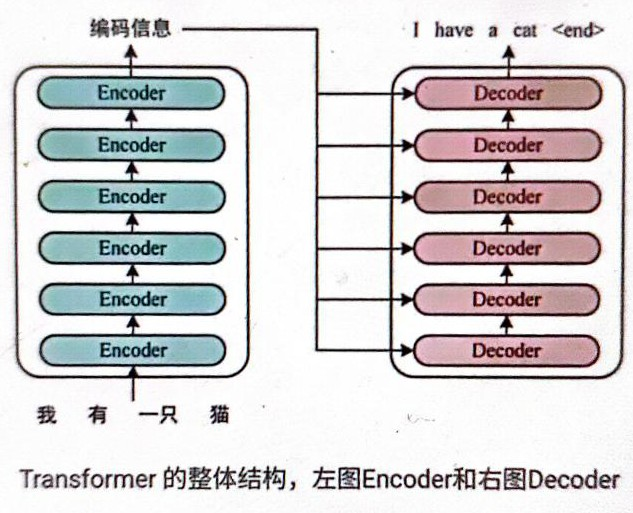
\includegraphics{images/image-0016.jpeg}
\caption{Transformer 的整体结构示意图}
\end{figure}

Transformer 的整体结构：左侧为 Encoder，右侧为 Decoder。

\begin{figure}[htbp]
\centering
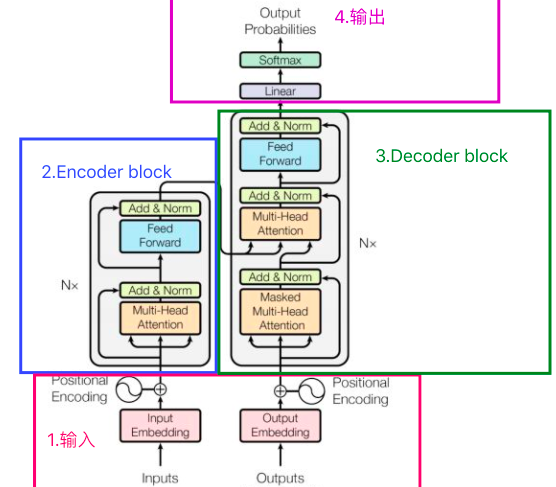
\includegraphics{images/image-0017.png}
\caption{Transformer 模块总览图}
\end{figure}

\hypertarget{ux4e00ux8f93ux5165}{%
\subsection{一、输入}\label{ux4e00ux8f93ux5165}}

\begin{enumerate}
\def\labelenumi{\arabic{enumi}.}
\item
  左下 inputs 表示输入序列，右下 Outputs (shifted right) 表示输出内容（其实是只提供该时间步以前生成的内容，训练预测能力）。
\item
  词嵌入 (Word Embedding)：每个词会被映射到一个固定长度的向量。例如，``猫''可能被表示为 \texttt{{[}0.1,\ -0.4,\ 0.8,\ ...{]}}。这些向量在训练开始时是随机的，模型会逐渐学习到让意思相近的词（如``猫''和``虎''）拥有更相似的向量。
\item
  位置编码 (Positional Encoding)：由于 Transformer 抛弃了 RNN 的顺序结构，后续的编码器本身无法感知词语的位置。没有位置信息，``我打你''和``你打我''在模型看来是一样的。为了解决这个问题，我们需要给每个词的向量中加入``位置信号''。后面会介绍位置编码。
\end{enumerate}

\hypertarget{ux4e8cencoder-block}{%
\subsection{二、Encoder Block}\label{ux4e8cencoder-block}}

\begin{enumerate}
\def\labelenumi{\arabic{enumi}.}
\item
  多头自注意力 (Multi-Head Attention)：编码器的核心，读取输入内容，通过多头自注意力机制，逐层得到富含上下文信息的中间表示。
\item
  Add：参照了残差神经网络，与输入直接相加。
\item
  Layer Normalization：对上一步的结果进行归一化处理。它能使模型训练过程更加稳定和快速，减少对参数初始化的敏感度。我们用 Layer Normalization (LN)，而不是 Batch Normalization (BN)，这二者的区别是：
\end{enumerate}

假设我们的输入数据形状为 {[}Batch\_Size, Seq\_Len, d\_model{]}，比如：{[}32, 10, 512{]}（32个句子，每句10个词，每个词512维）。

Batch Normalization (BN) 是``纵向切''，它固定特征维度，统计整个Batch的均值和方差。对于第i个特征维度（比如第0维），它会把这32个句子中、所有位置的词的第0维拿出来求平均。这在NLP中非常糟糕。因为不同句子的长度不同（通常靠Padding补齐），且不同位置的词语义差异极大，不同语段中各个特征维度的分布也往往有天然差异，强行让所有词语的第0维符合正态分布是不合理的，相当于``扭曲''了embedding空间，改变了向量之间的相似度，直接破坏embedding空间中存储的语义信息。

Layer Normalization (LN)是``横向切''，它固定样本（Token），统计该Token自身所有维度的均值和方差。对于第1个句子的第1个词（一个512维的向量），它计算这 512 个数值的均值和方差，然后进行伸缩，实质上抹平了向量模长的差异，让每个token的各个特征近似服从N(0,1)，这样点积就可以近似表示余弦相似度，即语义相似度。LN 将所有向量拉回到同一个``单位球壳''附近，让模型专注于学习方向（特征的组合方式，即语义），而不是数值的大小。

\begin{enumerate}
\def\labelenumi{\arabic{enumi}.}
\setcounter{enumi}{3}
\tightlist
\item
  Feed Forward：在每个注意力层之后，编码器和解码器都会有一个简单的前馈神经网络。这个网络对每个位置的向量独立地进行一次非线性变换。它由两个线性层和一个 ReLU 激活函数组成，可以看作是对注意力机制提取出的信息进行进一步的加工和提炼，增加模型的非线性能力。
\end{enumerate}

\hypertarget{ux4e09decoder-block}{%
\subsection{三、Decoder Block}\label{ux4e09decoder-block}}

\begin{enumerate}
\def\labelenumi{\arabic{enumi}.}
\tightlist
\item
  带掩码的多头自注意力 (Masked Multi-Head Self-Attention)
\end{enumerate}

（1）目的与工作方式：``回顾已写内容''。在生成下一个词时，解码器需要知道自己前面已经写了什么，以保证句子的连贯性。例如，已经写了 ``I am a''，下一个词很可能是 ``cat''，而不是重复生成 ``I''。它和编码器中的自注意力机制几乎完全一样，都是为了计算序列内部词与词之间的关系。

（2）为什么需要掩码？

在训练时，我们已经知道了完整的译文（例如 ``I am a cat''）。如果没有掩码，当模型在预测 ``am'' 这个词时，它会``偷看''到后面的 ``a'' 和 ``cat''，这显然是在作弊，模型学不到真正的预测能力。

（3）如何实现掩码？

掩码是一个``上三角矩阵''，它在计算注意力分数后、进行 Softmax 之前起作用。它会强制将所有未来位置 \((i,j)\)（\(i>j\)）的注意力分数，即 \(q_i\) 与 \(k_j\) 的点积设置为一个绝对值极大的负数（例如 \(-10^9\)）。

效果：绝对值极大的负数经过 Softmax 函数后，其对应的权重会无限接近于0。这样一来，模型在计算任意位置的输出时，其注意力权重只能分布在当前位置和之前的位置上，从而保证了模型无法``看到未来''。

\begin{enumerate}
\def\labelenumi{\arabic{enumi}.}
\setcounter{enumi}{1}
\tightlist
\item
  编码器-解码器注意力 (Encoder-Decoder Attention / Cross-Attention)
\end{enumerate}

（1）目的：这是连接编码器和解码器的核心桥梁。它让解码器在生成译文的每一步，都能去关注原文中最相关的部分。它用自己当前的理解(Q)去查询原文的完整信息 (K和V)，看看原文的哪一部分对生成下一个词最重要。

（2）工作方式：这也是一个多头注意力层，但它的 \(Q,K,V\) 来源不同：

查询向量 (Query, Q)：来自解码器前一个子层（即带掩码的自注意力层）的输出。这个 Q 向量代表了``写作部''当前的需求，可以理解为：``根据我已经写出的内容（比如 `I am'），我现在需要什么信息来决定下一个词？''

键向量 (Key, K) 和 值向量 (Value, V)：全部来自编码器栈的最终输出（即``理解部''的最终版精读笔记）。这两个向量代表了原文的完整信息，并且在解码的整个过程中是固定不变的。

（3）比喻：解码器（作者）拿着自己的草稿（Q 向量）去问编码器（原文摘要）：``我的草稿写到这了，请问你原文中哪部分内容跟我现在要写的最相关？'' 编码器通过 K, V 向量回答它，解码器据此获得生成下一个词的关键线索。例如，当解码器生成到与 ``猫'' 对应的位置时，这一层的注意力会高度集中在编码器输出中代表 ``猫'' 的那个向量上。

\begin{enumerate}
\def\labelenumi{\arabic{enumi}.}
\setcounter{enumi}{2}
\tightlist
\item
  前馈神经网络 (Position-wise Feed-Forward Network)
\end{enumerate}

（1）目的：``消化整合，深入思考''。

（2）工作方式：这个子层与编码器中的前馈网络完全相同。它接收来自编码器-解码器注意力层的输出向量，并对其进行一次非线性变换。

（3）比喻：在回顾了自己写的内容（Masked Self-Attention）并查阅了原文（Encoder-Decoder Attention）之后，解码器需要一个``独立思考''的过程，将这些信息进行整合、加工和提炼，最终形成一个准备用于预测下一个词的、信息高度浓缩的向量。这个``独立思考''的过程就是由前馈网络完成的。

\hypertarget{ux56dbux8f93ux51fa}{%
\subsection{四、输出}\label{ux56dbux8f93ux51fa}}

\begin{enumerate}
\def\labelenumi{\arabic{enumi}.}
\tightlist
\item
  取注意力层输出矩阵的什么内容？
\end{enumerate}

注意力层输出矩阵的形状为 \texttt{{[}seq\_len,d\_model{]}}，其中 \texttt{seq\_len} 是输入序列长度。

我们的目标是预测序列的 Next Token（如第4个词），我们只需要关注序列中最后一个 Token（第3个词）经过模型处理后的输出向量。因为在 Masked Self-Attention（带掩码的自注意力）机制下，最后一个 Token 的向量 \(h\) 已经聚合了整个序列的所有历史信息。

若希望得到原序列经过交互后富含上下文信息的序列：输出整个矩阵对应的Token序列。

\begin{enumerate}
\def\labelenumi{\arabic{enumi}.}
\setcounter{enumi}{1}
\tightlist
\item
  计算相似度
\end{enumerate}

得到输出向量后，我们会将其转化为输出 Token，具体操作为：和词表中所有 Token 计算点积相似度，这一步可以用矩阵乘法表示为 \(hW\)（\(W\) 是输出层的权重矩阵，每一行被视为词表中对应词的嵌入向量），经过 Softmax 后输出。

为什么可以用点积作为相似度呢？我们先从余弦相似度说起：

假设我们有两张不同的猫的图片，对应向量 \(x\) 和 \(y\)，我们希望它们的欧氏距离很小。在少数轮廓、皮毛之类的信号维度上，\(x_i\) 和 \(y_i\) 的值可能很相似，所以 \((x_i-y_i)^2\) 很小；但在草地、光照、拍摄角度等海量噪音维度上，\(x_i\) 和 \(y_i\) 会有微小的随机差异，每个 \((x_i-y_i)^2\) 可能不大，但它们的数量是压倒性的。

欧氏距离的 \(L_2\) 度量本质上是一个无差别的累加器：

\[
d^2(x,y)=\sum_{i\in\text{Signal}}(x_i-y_i)^2+\sum_{j\in\text{Noise}}(x_j-y_j)^2
\]

它将信号维度上的微小差异与海量噪音维度上的随机差异同等对待，并将它们的平方和累加起来。最终总距离的计算结果可能由噪音项的总和主导，因此并不适合作为高维语义向量的主要相似度度量。

余弦相似度衡量的是两个向量在方向上的接近程度，直接忽略它们的绝对长度：

\[
d_{\cos}(x,y)=\frac{x\cdot y}{\|x\|\|y\|}=\frac{\sum_{i=1}^{D}x_i y_i}{\sqrt{\sum_{i=1}^{D}x_i^2}\sqrt{\sum_{i=1}^{D}y_i^2}}
\]

方向是一种比长度更稳健的度量，承载了更纯净的各向异性信号：

\begin{itemize}
\tightlist
\item
  高维中随机的背景噪音几乎都是正交的，点积会非常接近 0。
\item
  而构成猫的信号维度在不同猫图片向量中表现出一致的方向性，点积可以增强这一点。
\end{itemize}

实际上，大模型中使用的多为点积相似度。原因：

（1）效率与简化计算\hspace{0pt}：点积运算 (A · B) 本身比余弦相似度计算（需要先计算点积，再除以两个向量的模长 \textbar\textbar A\textbar\textbar{} * \textbar\textbar B\textbar\textbar）更简单高效。在自回归生成中，模型需要为词表中的每一个词（通常是数万甚至数十万个）计算一个相似度分数，点积能显著减少计算量。

（2）与Softmax的天然配合：模型的学习过程已经内化了对向量``长度''的调整，各个向量长度几乎差不多。这时，点积计算得到的分数（通常称为 logits）会直接输入到 Softmax 函数中，以转换为下一个词的概率分布。所有词都除以模长或者都不除以模长对于经过 Softmax 函数后的概率分布没有影响，因此这一步可以被省略而不影响模型性能。

\begin{enumerate}
\def\labelenumi{\arabic{enumi}.}
\setcounter{enumi}{2}
\tightlist
\item
  自回归输出
\end{enumerate}

模型每次利用序列前文 \([x_1,\ldots,x_{i-1}]\) 作为输入，输出一个 token 即 \(x_i\)，再将 \([x_1,\ldots,x_i]\) 作为新的输入，以此类推。这个``输入 -\textgreater{} 解码器栈处理 -\textgreater{} 线性层 -\textgreater{} Softmax -\textgreater{} 选择词语''的循环会一直进行下去，直到选出的词是特殊的句子结束符 \texttt{\textless{}/s\textgreater{}} 为止。这个过程是串行的。

\hypertarget{ux53c2ux8003ux6587ux732e-68}{%
\subsection{参考文献}\label{ux53c2ux8003ux6587ux732e-68}}

\begin{itemize}
\tightlist
\item
  Vaswani, A., Shazeer, N., Parmar, N., et al.~(2017). \href{https://arxiv.org/abs/1706.03762}{Attention Is All You Need}. NeurIPS 2017.
\end{itemize}

\clearpage

\hypertarget{ux4f4dux7f6eux7f16ux7801}{%
\section{位置编码}\label{ux4f4dux7f6eux7f16ux7801}}

Transformer的标准处理流程中，并没有考虑token在序列的不同位置带来的差异。为了打上这个``补丁''，一般我们会运用基于正余弦的位置编码。

\hypertarget{ux4e00ux7ecfux5178transformerux7684ux6b63ux4f59ux5f26ux4f4dux7f6eux7f16ux7801}{%
\subsection{一、经典Transformer的正余弦位置编码}\label{ux4e00ux7ecfux5178transformerux7684ux6b63ux4f59ux5f26ux4f4dux7f6eux7f16ux7801}}

\hypertarget{ux4e00ux516cux5f0fux5f62ux5f0f}{%
\subsubsection{（一）公式形式}\label{ux4e00ux516cux5f0fux5f62ux5f0f}}

假设我们有一个输入序列，其长度为 \(L\)，模型的隐藏层维度（Embedding Dimension）为 \(d_{model}\)。对于序列中位置为 \(pos\) 的词（\(0 \le pos < L\)），以及该词向量中的第 \(i\) 个维度（\(0 \le i < d_{model}\)），其位置编码 \(PE\) 的计算公式如下：

\[
PE_{(pos,2i)}=\sin\left(\frac{pos}{10000^{2i/d_{model}}}\right)
\]

\[
PE_{(pos,2i+1)}=\cos\left(\frac{pos}{10000^{2i/d_{model}}}\right)
\]

对于每个位置，利用上面的函数可以生成一个位置向量，这个向量会和词的嵌入向量相加。``相加''意味着融合，模型在学习 token 的信息时，也同时学习到了位置信息。

\hypertarget{ux4e8cux539fux7406ux89e3ux91ca}{%
\subsubsection{（二）原理解释}\label{ux4e8cux539fux7406ux89e3ux91ca}}

\begin{enumerate}
\def\labelenumi{\arabic{enumi}.}
\tightlist
\item
  为什么使用正余弦？
\end{enumerate}

（1）有界性：位置编码向量的每一维都被控制在 \([-1,1]\)，不至于``喧宾夺主''压倒语义信息。

（2）对不同长度序列的适应性：

假设我们设定一个最大长度 \(L_{max}\)，位置 \(pos\) 的编码为：

\[
PE(pos)=\frac{pos}{L_{max}}
\]

如果 \(L_{max}\) 是针对当前句子长度动态设定的，就会出现致命缺陷：步长不一致。例如句子 A 长度为 5，第 1 个词是 0.0，第 2 个词是 0.2，相邻距离是 0.2；句子 B 长度为 100，第 1 个词是 0.0，第 2 个词是 0.01，相邻距离是 0.01。模型无法稳定学习``相邻''这个概念。

如果 \(L_{max}\) 是全局固定的极大值（比如 10000），当 \(L_{max}\) 很大时，相邻两个位置的差异 \(\Delta=\frac{1}{10000}\) 会非常微小。在深层神经网络中，这样微小的数值差异很容易被噪声淹没，导致模型很难区分位置 100 和位置 101。相比之下，正弦编码在高频分量上的数值变化非常剧烈，更容易区分相邻位置。

（3）位置可加性：由三角函数的性质

\[
\sin(\alpha+\beta)=\sin\alpha\cos\beta+\cos\alpha\sin\beta
\]

\[
\cos(\alpha+\beta)=\cos\alpha\cos\beta-\sin\alpha\sin\beta
\]

因此：

\[
\begin{pmatrix}
PE_{(pos+k,2i)} \\
PE_{(pos+k,2i+1)}
\end{pmatrix}
=
\begin{pmatrix}
\cos(\omega_i k) & \sin(\omega_i k) \\
-\sin(\omega_i k) & \cos(\omega_i k)
\end{pmatrix}
\begin{pmatrix}
PE_{(pos,2i)} \\
PE_{(pos,2i+1)}
\end{pmatrix}
\]

这是一个标准的旋转矩阵（Rotation Matrix）。结论是，\(PE_{(pos+k)}\) 确实可以由 \(PE_{(pos)}\) 乘以一个与 \(pos\) 无关、仅与 \(k\) 有关的线性变换矩阵得到。这使得 Self-Attention 机制能够很容易地学会关注``距离当前词 \(k\) 个单位''的词，即具备了捕捉相对位置的能力。

\begin{enumerate}
\def\labelenumi{\arabic{enumi}.}
\setcounter{enumi}{1}
\tightlist
\item
  为什么位置编码是一个 \(d_{model}\) 维的向量，对于每一个特征维度 \(i\) 都不一样？
\end{enumerate}

首先明确：虽然语义编码和位置编码维数相同，但二者的第i维之间没有物理意义上的一一对应。

为什么位置编码需要 \(d_{model}\) 维呢？这是因为在一个长序列中，如果只用一维表征信息，会出现严重的问题。比如序列有一百万个 token，那么在一圈弧度为 \(2\pi\) 的情况下，第 5 个和第 15 个 token 之间的角度就是 \(2 \times 10^{-5}\pi\)，在三角函数运算后差距几乎为零，淹没在随机噪声中。

同时，让所有维度的位置编码都用同一个值还会带来两个问题。首先是会让语义向量沿 \((1,1,\ldots)\) 的统一方向移动，而这个方向可能本来要表征其他语义。其次是 Layer Normalization 过程中会对每个向量进行归一化：

\[
\mathrm{LN}(x)=\frac{x-\mu}{\sigma}\cdot\gamma+\beta
\]

这会直接把位置编码``清洗''掉。

因此，我们需要增加维度。就像一个一位布尔值只能表示 0 或 1，但是八位编码却能表示 256 个数值。利用三角函数的旋转特性，我们想到可以用一个有 \(d_{model}\) 根指针的``时钟''，将编码的高位数存在低频率旋转的``时针''中，低位数存在高频率旋转的``秒针''中：

我们可以将分母 \(10000^{2i/d_{model}}\) 理解为波长，或者将其倒数理解为频率。令频率 \(\omega_i=\frac{1}{10000^{2i/d_{model}}}\)，则公式可简化为：

\[
PE_{(pos,2i)}=\sin(\omega_i\cdot pos)
\]

\[
PE_{(pos,2i+1)}=\cos(\omega_i\cdot pos)
\]

\begin{itemize}
\tightlist
\item
  低维度（\(i\) 较小）：\(\omega_i\) 较大，波长短，变化频率高。
\item
  高维度（\(i\) 较大）：\(\omega_i\) 极小，波长极长，变化频率低。
\end{itemize}

在 Transformer 的公式中，分母 \(10000^{2i/d}\) 就是波长 \(\lambda_i\)。例如：

\begin{itemize}
\tightlist
\item
  当 \(i=0\)（第 0 维）时，分母是 \(10000^0=1\)。这是一个超短波，\(pos\) 每增加 \(2\pi\)（约 6 个词），正弦波就跑完一整圈。作用：它像一把``游标卡尺''，负责精确区分相邻的、微小的位置变化（比如 \(pos=5\) 和 \(pos=6\)）。
\item
  当 \(i=256\)（第 512 维）时，分母是 \(10000^1=10000\)。这是一个超长波，\(pos\) 需要增加 \(10000\cdot2\pi\)（约 6 万个词），正弦波才跑完一圈。作用：它像一把``公里计数器''，在短句子里几乎是一条直线，负责提供宏观的、全局的定位。
\end{itemize}

\begin{enumerate}
\def\labelenumi{\arabic{enumi}.}
\setcounter{enumi}{2}
\tightlist
\item
  为什么波长不能线性增长，而要用 \(10000^{2i/d}\) 这种指数形式？
\end{enumerate}

想象你要用几个数字转盘来表示从 0 到 10000 的数字：

\begin{itemize}
\tightlist
\item
  线性方案（极低效）：如果你有 3 个转盘，分别代表 1s、2s、3s，你能表示的范围非常窄，或者你需要成千上万个转盘才能数到 10000。
\item
  指数方案（十进制/位值制）：你有 3 个转盘，分别代表：

  \begin{itemize}
  \tightlist
  \item
    转盘 A：\(10^0=1\)（个位）
  \item
    转盘 B：\(10^1=10\)（十位）
  \item
    转盘 C：\(10^2=100\)（百位）
  \end{itemize}
\end{itemize}

注意到了吗？1、10、100 就是指数级增长的。仅仅用 3 个维度（个、十、百），我们就能覆盖很大的范围，而且每个数字的表示都是唯一的。

Transformer 的 512 个维度也是这个道理：我们不希望第 10 维和第 11 维的波长差不多（比如 50 和 51），那样太浪费了。我们希望它们成倍增长。通过指数级的波长分配，512 个维度均匀地覆盖了从 \(2\pi\) 到 \(10000\cdot2\pi\) 的巨大范围，这让模型在对数尺度（Log Scale）上拥有了均匀的分辨率。

\hypertarget{ux4e8cux65cbux8f6cux4f4dux7f6eux7f16ux7801rope}{%
\subsection{二、旋转位置编码（RoPE）}\label{ux4e8cux65cbux8f6cux4f4dux7f6eux7f16ux7801rope}}

RoPE 是目前各大主流语言模型（如 LLaMA、Qwen）标配的位置编码方式。它不像上面那样直接``加上''一个位置向量，而是通过在复平面上的``旋转''来注入位置信息，从而自带相对位置信息的感知能力。

对于一个位置为 \(m\) 的输入向量 \(x=[x_1,x_2,\ldots,x_d]^T\)，RoPE 将相邻的两个维度视为一组二维坐标，并根据位置 \(m\) 乘以一个旋转矩阵。其完整的块对角旋转矩阵 \(R_{\Theta,m}^{d}\) 表达式如下：

\[
\begin{pmatrix}
\cos(m\theta_1) & -\sin(m\theta_1) & 0 & 0 & \cdots & 0 & 0 \\
\sin(m\theta_1) & \cos(m\theta_1) & 0 & 0 & \cdots & 0 & 0 \\
0 & 0 & \cos(m\theta_2) & -\sin(m\theta_2) & \cdots & 0 & 0 \\
0 & 0 & \sin(m\theta_2) & \cos(m\theta_2) & \cdots & 0 & 0 \\
\vdots & \vdots & \vdots & \vdots & \ddots & \vdots & \vdots \\
0 & 0 & 0 & 0 & \cdots & \cos(m\theta_{d/2}) & -\sin(m\theta_{d/2}) \\
0 & 0 & 0 & 0 & \cdots & \sin(m\theta_{d/2}) & \cos(m\theta_{d/2})
\end{pmatrix}
\]

其中，旋转角 \(\theta_i=10000^{-2(i-1)/d}\)。最终注入了位置信息的特征向量即为 \(x'_m=R_{\Theta,m}^{d}x\)。

对于非一维的序列（如视频），既然视频是 3D 数据（时间、高度、宽度），V-JEPA 2 采用的是 1D-RoPE 的 3D 扩展版本。具体的做法是：将总的特征维度 \(d\) 平分为三个大致相等的部分：\(d_t\)（时间轴）、\(d_h\)（高度轴）和 \(d_w\)（宽度轴）。对于视频中的某一个 Patch，假设它在时间帧上的坐标为 \(t\)，空间坐标为 \((h,w)\)，则分别对这三个特征分段应用对应维度的 1D 旋转。

\hypertarget{ux53c2ux8003ux6587ux732e-69}{%
\subsection{参考文献}\label{ux53c2ux8003ux6587ux732e-69}}

\begin{itemize}
\tightlist
\item
  Vaswani, A., Shazeer, N., Parmar, N., et al.~(2017). \href{https://arxiv.org/abs/1706.03762}{Attention Is All You Need}. NeurIPS 2017.
\item
  Su, J., Lu, Y., Pan, S., Wen, B., \& Liu, Y. (2021). \href{https://arxiv.org/abs/2104.09864}{RoFormer: Enhanced Transformer with Rotary Position Embedding}. arXiv:2104.09864.
\end{itemize}

\clearpage

\hypertarget{bert}{%
\section{BERT}\label{bert}}

\hypertarget{ux4e00ux6838ux5fc3ux601dux60f3ux57faux4e8etransformerux7684ux53ccux5411ux4e0aux4e0bux6587ux7f16ux7801ux5668}{%
\subsection{一、核心思想：基于Transformer的双向上下文编码器}\label{ux4e00ux6838ux5fc3ux601dux60f3ux57faux4e8etransformerux7684ux53ccux5411ux4e0aux4e0bux6587ux7f16ux7801ux5668}}

BERT的核心思想在于：要真正理解一个词的含义，必须同时考虑它左右两侧的所有上下文。它通过一种称为~``双向编码器''~的架构来实现这一点。BERT的模型架构基础是Google在2017年提出的Transformer模型，但BERT只使用了Transformer的编码器部分，BERT-base模型由12层Transformer编码器堆叠而成，BERT-large则有24层。

注意力机制是Transformer的核心，也是BERT实现双向理解的关键。它允许序列中的任何一个词直接与序列中的所有其他词进行交互，计算它们之间的关联权重。通过这种方式，模型在处理每个词时，都``注意''到了整个句子的信息。此外，在输入词的嵌入向量中加入了位置编码，告诉模型每个词在序列中的具体位置。

\hypertarget{ux4e8cux5173ux952eux6280ux672fux4e24ux5927ux9884ux8badux7ec3ux4efbux52a1}{%
\subsection{二、关键技术：两大预训练任务}\label{ux4e8cux5173ux952eux6280ux672fux4e24ux5927ux9884ux8badux7ec3ux4efbux52a1}}

BERT的强大能力还来自其开创性的预训练方法。它在海量无标注文本上通过两个巧妙的``完形填空''任务进行训练，从而学习到通用的语言表示。一般以下两个任务同时进行。

\begin{enumerate}
\def\labelenumi{\arabic{enumi}.}
\tightlist
\item
  掩码语言模型（Masked Language Model, MLM）
\end{enumerate}

操作：在输入序列中，随机地遮盖（Mask）掉15\%的词语（用~{[}MASK{]}~标记替换）。

任务：模型的任务是预测这些被遮盖的原始词语是什么。

目的：这一步是实现BERT``双向性''的关键。这种方法强制模型必须根据上下文中的所有词（包括被遮盖词左右两边的词）来重建被遮盖的词，从而学会了深层的双向语言表征。

技巧：在这15\%的被选中的词中，并不是全部替换为~{[}MASK{]}。80\%的时间替换为~{[}MASK{]}；10\%的时间替换为一个随机的词，引入噪声，防止模型过于``自信''，增强模型的鲁棒性；10\%的时间保持原词不变，因为在微调阶段，输入的都是真实的、未被修改的词语。这10\%的情况让模型在预训练时也能接触到完整的、未被破坏的原始句子，使得预训练和微调的数据环境更加接近，也让模型知道``苹果''在这个上下文中是合理的，并且需要为其生成一个好的上下文向量表示。

改进：Span-Mask

BERT 的预训练目标（Masked Language Model, MLM）是随机选择序列中 15\% 的单个 token（令牌，可以理解为单词或子词），然后用 {[}MASK{]} 标签替换它们。如The quick brown {[}MASK{]} jumps {[}MASK{]} the lazy dog.模型需要独立地预测每个 {[}MASK{]} 位置上原来的 token (例如 fox 和 over)，可以利用 jumps 和 the 来预测 over，而不需要真正理解 jumps over 这个短语的含义。

Span-Mask的改进是，这种方法不再掩盖单个、分散的 token，而是选择一个连续的文本``跨度''（Span），并将这个连续片段中的所有 token 都替换掉。如假设我们要掩盖 quick brown fox 这个 span，输入The {[}MASK{]} {[}MASK{]} {[}MASK{]} jumps over the lazy dog.模型现在必须一次性地重建整个被掩盖的 quick brown fox 片段，模型不仅要预测被掩盖的 token 是什么，还必须知道内部结构（预测出 quick、brown 和 fox 之间的顺序和关系）以及跨度长度（模型需要学习到它应该生成三个 token 来填补这个空白，而不是一个或两个）。

总之，这可以强迫模型学习更丰富的上下文信息、序列的内部结构以及被掩盖片段的长度。这被认为是一个比标准 BERT 的 MLM 更难、也更有效的预训练任务。比如，对于蛋白质序列来说，这意味着模型不是在预测单个被掩盖的氨基酸，而是在预测一个连续的氨基酸片段，这可能迫使模型更好地学习蛋白质的局部结构或功能基序 (motif)。

\begin{enumerate}
\def\labelenumi{\arabic{enumi}.}
\setcounter{enumi}{1}
\tightlist
\item
  下一句预测（Next Sentence Prediction, NSP）
\end{enumerate}

为了让模型理解句子之间的关系（这对于问答、自然语言推理等任务至关重要），BERT增加了这个任务。

操作：在训练时，给模型输入两个句子A和B，其中50\%的情况下B是A的真实下一句（标签为~IsNext），另外50\%的情况下B是从语料库中随机抽取的（标签为~NotNext）。

任务：模型需要判断句子B是否是句子A的下一句。

目的：使模型能够捕捉两个文本片段之间的逻辑和语义关系。

\hypertarget{ux4e09ux5faeux8c03ux65b9ux5f0f}{%
\subsection{三、微调方式}\label{ux4e09ux5faeux8c03ux65b9ux5f0f}}

由于BERT本质是一个编码器，所以将其运用于特定的下游任务（如情感分类、问答、命名实体识别）时，只需要在BERT后面加一个简单的输出层（如一个全连接层），使用有标签的任务数据对这个模型进行端到端的精细调整即可。由于模型已经在通用语言上有了很好的基础，只需要少量数据微调就能在特定任务上取得极佳的效果。

\hypertarget{ux56dbux8f93ux5165ux8868ux793a}{%
\subsection{四、输入表示}\label{ux56dbux8f93ux5165ux8868ux793a}}

BERT的输入能够统一表示一个句子或一个句子对（如\textless 问题，答案\textgreater）。输入序列由三种嵌入向量求和而成：

词嵌入：将每个词转换成的向量。

段落嵌入：一个学习到的向量，用于区分句子A和句子B。例如，句子A的所有词都用~EA，句子B的所有词都用~EB。

位置嵌入：表示每个词在序列中位置信息的向量。

此外，每个序列的开头都有一个特殊的~{[}CLS{]}~标记，该标记的最终输出向量常用于分类任务（如情感分析）。句子之间用~{[}SEP{]}~标记分隔。

\hypertarget{ux4e94ux8f93ux51faux8868ux793aux591aux5c42ux7ea7ux7684ux8bedux4e49ux5411ux91cf}{%
\subsection{五、输出表示：多层级的语义向量}\label{ux4e94ux8f93ux51faux8868ux793aux591aux5c42ux7ea7ux7684ux8bedux4e49ux5411ux91cf}}

经过L层（BERT-base为12层）Transformer编码器的复杂计算与交互后，BERT最终会输出一个包含了丰富语义信息的张量。这个输出根据下游任务的需求，主要分为两种形式：

\begin{enumerate}
\def\labelenumi{\arabic{enumi}.}
\tightlist
\item
  序列输出
\end{enumerate}

这是BERT最基础、最原本的输出形式。假设输入序列的长度为N（包含{[}CLS{]}和{[}SEP{]}标记），隐藏层的维度为d\_model（BERT-base为768）。那么，序列输出可以表示为一个N*d\_model维矩阵：H = {[}h\_CLS, h\_1, h\_2, \ldots, h\_n, h\_SEP{]}，每一个h\_i都是一个维度为768的上下文相关的动态词向量。由于注意力机制的存在，向量h\_i虽然对应位置i的词，但它实际上融合了整个句子中所有其他词的信息。例如，在``苹果掉在地上''和``苹果手机发布会''中，尽管输入都是``苹果''，但输出的对应向量h\_apple是完全不同的。

适用任务：适用于词/Token级别的任务，如命名实体识别（对每个词进行分类）、问答系统（寻找答案在文章中的``起始位置''和``结束位置''）等。

\begin{enumerate}
\def\labelenumi{\arabic{enumi}.}
\setcounter{enumi}{1}
\tightlist
\item
  池化输出
\end{enumerate}

BERT使用序列第一个位置的特殊标记{[}CLS{]}的最终向量h\_CLS来代表整个句子的语义，它是一个高度压缩的、融合了全句核心意图的向量，是整个输入序列的``身份证''。一般会让h\_CLS再经过一个``池化层''，包括一个全连接层和tanh 激活函数，以让输出更适合作为分类任务的特征。

适用任务：适用于句子级别（Sentence-level）的任务，如：情感分析（判断句子是褒义还是贬义）、句子关系判断、下一句预测等。

\hypertarget{ux53c2ux8003ux6587ux732e-70}{%
\subsection{参考文献}\label{ux53c2ux8003ux6587ux732e-70}}

\begin{itemize}
\tightlist
\item
  Devlin, J., Chang, M.-W., Lee, K., \& Toutanova, K. (2019). \href{https://arxiv.org/abs/1810.04805}{BERT: Pre-training of Deep Bidirectional Transformers for Language Understanding}. NAACL 2019.
\item
  Joshi, M., Chen, D., Liu, Y., Weld, D. S., Zettlemoyer, L., \& Levy, O. (2020). \href{https://arxiv.org/abs/1907.10529}{SpanBERT: Improving Pre-training by Representing and Predicting Spans}. TACL.
\end{itemize}

\clearpage

\hypertarget{ux6ce8ux610fux529bux673aux5236ux4e0eux68afux5ea6ux4e0bux964dux7684ux7b49ux4ef7ux6027}{%
\section{注意力机制与梯度下降的等价性}\label{ux6ce8ux610fux529bux673aux5236ux4e0eux68afux5ea6ux4e0bux964dux7684ux7b49ux4ef7ux6027}}

注意力模块Transformer的Attention层（包含残差流在内）整体上可以被看作是一种回归问题的梯度下降优化。

\hypertarget{ux4e00ux7ebfux6027ux6ce8ux610fux529bux7684ux8868ux8fbeux5f0f}{%
\subsection{一、线性注意力的表达式}\label{ux4e00ux7ebfux6027ux6ce8ux610fux529bux7684ux8868ux8fbeux5f0f}}

对于一组token（模型输入序列）\(`\{e_1,\ldots,e_n\}`\) 和 query（test）token \(`e_{\mathrm{test}}`\)，经过去除Softmax的注意力层（即线性注意力层，后面会探讨加上Softmax的情形）后，注意力的表达式为：

\[
\mathrm{Output}_{\mathrm{test}}=e_{\mathrm{test}}+PVK^\top q_{\mathrm{test}}
\tag{1}
\]

其中输出加上自身是因为残差连接；\(`P`\) 为输出投影矩阵。若我们将 \(`V`\) 视为 \(`(v_1,\ldots,v_t)`\)，\(`K`\) 视为 \(`(k_1,\ldots,k_t)`\)，则 \(`VK^\top=\sum_i v_i k_i^\top`\)，即：

\[
\mathrm{Output}_{\mathrm{test}}=e_{\mathrm{test}}+P\sum_i v_i k_i^\top q_{\mathrm{test}}
\tag{2}
\]

用类似RNN的方式表述即为：

\[
S_t=S_{t-1}+v_t k_t^\top
\]

\[
\mathrm{Output}_t=\mathrm{input}_t+PS_tq_t
\]

上式意味着，我们利用隐状态矩阵 \(`S`\) 构建了一个从 \(`K`\) 到 \(`V`\) 的映射，并获取在输入 \(`q_t`\) 时的输出，作为残差相加。忽略投影 \(`P`\)，这里的 \(`V`\) 实质上拟合的是``输出与输入之间的残差''。

\hypertarget{ux4e8cux6784ux9020ux7ebfux6027ux6a21ux578bux5e76ux8bc1ux660eux7b49ux4ef7ux6027}{%
\subsection{二、构造线性模型，并证明等价性}\label{ux4e8cux6784ux9020ux7ebfux6027ux6a21ux578bux5e76ux8bc1ux660eux7b49ux4ef7ux6027}}

假设我们正在进行 In-Context Learning（上下文学习），输入是一系列示例（演示数据）：\(`(x_1,y_1),(x_2,y_2),\ldots,(x_N,y_N)`\)，以及一个新的查询输入 \(`x_{\mathrm{test}}`\)。

在 Transformer 中，每个 Token 会将输入特征和标签拼接在一起。我们定义上下文矩阵为：

\[
X=[x_1,x_2,\ldots,x_N],\qquad Y=[y_1,y_2,\ldots,y_N]
\]

\textbf{输入 Token：} 假设将输入特征 \(`x_i`\) 和目标标签 \(`y_i`\) 拼接成一个列向量作为 token，即：

\[
e_i=\begin{pmatrix}x_i\\\\y_i\end{pmatrix}
\]

引入一个由权重矩阵 \(`W\in\mathbb{R}^{N_y\times N_x}`\) 参数化的参考线性模型 \(`y(x)=Wx`\)，以及一个包含输入样本 \(`x_i`\) 和标签 \(`y_i`\) 的训练数据集 \(`D=\{(x_i,y_i)\}_{i=1}^{N}`\)。学习的目标是最小化平方误差损失：

\[
L(W)=\frac{1}{2N}\sum_{i=1}^{N}\|Wx_i-y_i\|^2
\]

此时梯度下降的表达式（动态模型的更新方式）为：

\[
\Delta W=-\eta\nabla_W L(W)=-\frac{\eta}{N}\sum_{i=1}^{N}(Wx_i-y_i)x_i^\top
\tag{3}
\]

这里的 \(`Wx_i-y_i`\) 和前面的 \(`v_i`\) 对应（而不是 \(`y_i`\) 和 \(`v_i`\) 对应），表示``按原始权重的输出（\(`W_0x_i`\)）和应输出的值（标签 \(`y_i`\)）的差距''；\(`x_i`\) 和前面的 \(`k_i`\) 对应；\(`\eta/N`\) 和前面的 \(`P`\) 对应。这也就意味着，每次输入一批样本，\(`W`\) 的权重就将变化 \(`-P\sum_i v_i k_i^\top`\)。

也就是说，这个权重矩阵 \(`W`\) 和前面讲的隐状态矩阵 \(`S`\) 不一样：\(`W`\) 是隐式的，表示 \(`x`\) 到最终 \(`y`\) 的映射；\(`S`\) 是显式的，表示 \(`k`\) 到 \(`v`\)（残差 \(`Wx-y`\)）的映射。\(`\Delta W`\) 和 \(`S`\) 成比例关系，\(`W`\) 的一次梯度下降相当于运用了 \(`S`\) 中存储的所有上下文token的梯度。\(`(W+\Delta W)x_{\mathrm{test}}`\) 和 \(`\mathrm{input}_t+S_tq_t`\) 相对应。

对于测试token：

\[
e_{\mathrm{test}}=\begin{pmatrix}x_{\mathrm{test}}\\\\y_{\mathrm{init}}\end{pmatrix}
\]

我们初始化 \(`y_{\mathrm{init}}`\) 为 \(`-W_0x_{\mathrm{test}}`\)（后面会阐释为什么可以这么做）。通过构造 \(`W_Q`\)、\(`W_K`\)、\(`W_V`\) 矩阵，使得：

当前查询 token \(`j`\) 的 Query 向量：

\[
q_j=W_Q e_j=\begin{pmatrix}I_x&0\\\\0&0\end{pmatrix}\begin{pmatrix}x_j\\\\y_j\end{pmatrix}=\begin{pmatrix}x_j\\\\0\end{pmatrix}
\]

上下文 token \(`i`\) 的 Key 向量：

\[
k_i=W_K e_i=\begin{pmatrix}I_x&0\\\\0&0\end{pmatrix}\begin{pmatrix}x_i\\\\y_i\end{pmatrix}=\begin{pmatrix}x_i\\\\0\end{pmatrix}
\]

上下文 token \(`i`\) 的 Value 向量：

\[
v_i=W_V e_i=\begin{pmatrix}0&0\\\\W_0&-I_y\end{pmatrix}\begin{pmatrix}x_i\\\\y_i\end{pmatrix}=\begin{pmatrix}0\\\\W_0x_i-y_i\end{pmatrix}
\]

计算注意力：

\[
k_i^\top q_j=(x_i^\top,0)\begin{pmatrix}x_j\\\\0\end{pmatrix}=x_i^\top x_j
\]

\[
\sum_{i=1}^{N}v_i(k_i^\top q_j)=\sum_{i=1}^{N}\begin{pmatrix}0\\\\W_0x_i-y_i\end{pmatrix}(x_i^\top x_j)
\]

\[
PVK^\top q_j=\begin{pmatrix}\eta/N&0\end{pmatrix}\left(\sum_{i=1}^{N}(W_0x_i-y_i)x_i^\top x_j\right)
\]

这意味着对上下文中的 \(`W_0x-y`\) 进行``聚合''，可以视为得到的是 \(`W_0x_{\mathrm{test}}-y_{\mathrm{test}}`\)。我们想要的就是这个上下文聚合后得到的 \(`y`\) 值预测 \(`y_{\mathrm{test}}=(W_0+\Delta W)x_{\mathrm{test}}`\)，从而上式的下面部分就可以视为 \(`W_0x_{\mathrm{test}}-y_{\mathrm{test}}=-\Delta W x_{\mathrm{test}}`\)，也就是``原有输出-应然输出''。而这恰好和前面 \(`\Delta W`\) 的表达式对上了，因此：

\[
PVK^\top q_j=\begin{pmatrix}0\\\\-\Delta W x_j\end{pmatrix}
\]

这意味着对于test token，（1）式等价于：

\[
\mathrm{Output}
=\begin{pmatrix}x_{\mathrm{test}}\\\\-W_0x_{\mathrm{test}}\end{pmatrix}
+\begin{pmatrix}0\\\\-\Delta W x_{\mathrm{test}}\end{pmatrix}
=\begin{pmatrix}x_{\mathrm{test}}\\\\-(W_0+\Delta W)x_{\mathrm{test}}\end{pmatrix}
\tag{4}
\]

这条式子的下面部分取相反数后，也就得到参数变换后（按 \(`W_0+\Delta W`\)）应该输出的值，即注意力模块的输出。

\hypertarget{ux4e09ux4e3aux4ec0ux4e484ux5f0fux6709ux8d1fux53f7ux660eux660e-y_mathrmtestwx_mathrmtestdelta-wx_mathrmtestux4e3aux4ec0ux4e48ux8fd9ux91ccux662fux51cfux53bb-delta-wx_mathrmtest}{%
\subsection{\texorpdfstring{三、为什么（4）式有负号，明明 \(`y_{\mathrm{test}}=Wx_{\mathrm{test}}+\Delta Wx_{\mathrm{test}}`\)，为什么这里是减去 \(`\Delta Wx_{\mathrm{test}}`\)？}{三、为什么（4）式有负号，明明 `y\_\{\textbackslash mathrm\{test\}\}=Wx\_\{\textbackslash mathrm\{test\}\}+\textbackslash Delta Wx\_\{\textbackslash mathrm\{test\}\}`，为什么这里是减去 `\textbackslash Delta Wx\_\{\textbackslash mathrm\{test\}\}`？}}\label{ux4e09ux4e3aux4ec0ux4e484ux5f0fux6709ux8d1fux53f7ux660eux660e-y_mathrmtestwx_mathrmtestdelta-wx_mathrmtestux4e3aux4ec0ux4e48ux8fd9ux91ccux662fux51cfux53bb-delta-wx_mathrmtest}}

这需要从多轮优化的角度分析。大模型中往往是多个注意力层串行处理数据，每一轮都把输入 \(`x_{\mathrm{test}}`\) 转变为输出 \(`y_{\mathrm{test}}`\)，它又作为新的 \(`x_{\mathrm{test}}`\) 输入下一个注意力层。这等价于对一个线性层进行多轮权重更新：刚开始输入 \(`x_{\mathrm{test}}`\) 时（权重 \(`W_0`\)）执行一次梯度下降（权重变为 \(`W_0+\Delta W`\)）并输出 \(`y_{\mathrm{test}}`\)，它又作为新的 \(`x_{\mathrm{test}}`\) 输入（其他 \(`x_i`\) 和 \(`y_i`\) 仍然取原来的值）此时权重已经变为 \(`W_0+\Delta W`\) 的模型，再结合上下文进行梯度下降、推理，以此类推。

以上模型确实是正确的等价，但我们知道，实际上Transformer的权重是不变的，因此我们试图将上述过程再做一个等价转换，让 \(`W`\) 不变，而上下文 \(`y_i`\) 可变，更符合Transformer本身静态结构对应的表达式（即（1）式）。除了计算输出值（这一点我们已经有办法了）外，``当下的 \(`W`\) 值''唯一的``用处''就是用于梯度下降，而由（3）式可知，线性层梯度下降的幅度和残差 \(`Wx_i-y_i`\) 成正比，因此 \(`W`\) 从 \(`W_0`\) 变为 \(`W_0+\Delta W`\)，等价于上下文token的标签 \(`y_i`\) 减少 \(`\Delta Wx_i`\)，这时Loss不变，残差不变，优化状态不变。因此，我们可以假设多个线性层串行组成模型，每个线性层的参数均为 \(`W`\)，改变上下文token的 \(`y_i`\)：

\[
y_i^{new}=y_i-\Delta W x_i
\]

下一层的 \(`W`\) 不改变，但是这时候上下文token里输入的不是原始的 \(`y_i`\)，而是 \(`y_i^{new}`\)，下一层再对 \(`y_i^{new}`\) 进行类似的处理，以此类推，就可以通过改变上下文来等价地实现改变权重。

但是这时候会出现一个问题：自注意力层不会区分上下文token和test token，我们为了保证残差不变，把 \(`y_i`\) 减去 \(`\Delta Wx_i`\)，但是 \(`y_{\mathrm{test}}=W_0x_{\mathrm{test}}+\Delta Wx_{\mathrm{test}}`\)，符号反了。于是我们把 \(`y_{\mathrm{init}}`\) 取为 \(`-W_0x_{\mathrm{test}}`\)，减去 \(`\Delta Wx_{\mathrm{test}}`\) 后恰好为 \(`-W_0x_{\mathrm{test}}-\Delta Wx_{\mathrm{test}}`\)，乘以一个对角线全 \(`-1`\) 的输出投影矩阵即可。

\begin{figure}[htbp]
\centering
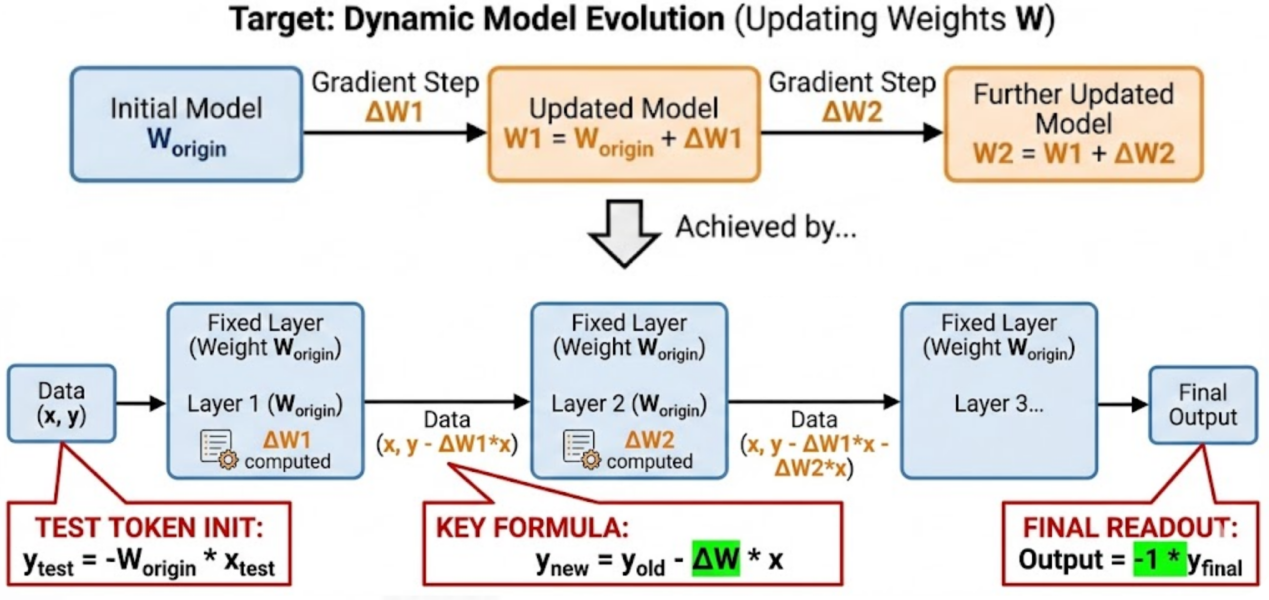
\includegraphics{images/image-0018.png}
\caption{动态权重更新与固定 Transformer 层的数据流等价关系}
\end{figure}

\begin{itemize}
\tightlist
\item
  穿过第 1 层注意力层（执行第 1 步梯度下降）：第 1 层根据当前的上下文计算出梯度增量 \(`\Delta W_1`\)。残差连接将其加上：
\end{itemize}

\[
y_{1,test}=y_{0,test}-\Delta W_1x_{\mathrm{test}}=-(W_0+\Delta W_1)x_{\mathrm{test}}
\]

\begin{itemize}
\tightlist
\item
  穿过第 2 层注意力层（执行第 2 步梯度下降）：第 2 层读取到 \(`y_{1,test}`\)，继续计算出新的梯度增量 \(`\Delta W_2`\)。残差连接再次将其加上：
\end{itemize}

\[
y_{2,test}=y_{1,test}-\Delta W_2x_{\mathrm{test}}=-(W_0+\Delta W_1+\Delta W_2)x_{\mathrm{test}}
\]

\begin{itemize}
\tightlist
\item
  穿过第 \(`K`\) 层注意力层（执行第 \(`K`\) 步梯度下降）：以此类推，经过 \(`K`\) 层后，测试 Token 的 \(`y`\) 值变成了：
\end{itemize}

\[
y_{K,test}=-W_0x_{\mathrm{test}}-\sum_{k=1}^{K}\Delta W_k x_{\mathrm{test}}
\]

\[
\hat{y}_{\mathrm{final}}=-y_{K,test}=W_0x_{\mathrm{test}}+\sum_{k=1}^{K}\Delta W_k x_{\mathrm{test}}
\]

这样，我们就把一个持续梯度下降的线性模型等价转化为了多个权重不变的线性层，数据在层间单向流动，每流过一个层，所有token（包括上下文token和test token）对应的 \(`y`\) 值都会减去 \(`\Delta Wx`\)，每一个这样的层就和Transformer中的每一个注意力层一一对应。值得注意的是，这样的 \(`W_0`\) 并非显式储存于Transformer的权重中，而是被隐式维护（虽然它也是不变的）：在前面的推理中，我们构造过：

\[
W_V=\begin{pmatrix}0&0\\\\W_0&-I_y\end{pmatrix}
\]

也就是说这里它由 \(`W_V`\) 决定。

总结：标准Transformer 无法在内部凭空变出一个真正的权重矩阵W存起来，只能靠修改数据流（残差）来``模拟''梯度下降，为了在多层Transformer中保证优化状态一致性，才采用了这种``别扭''的方式。

\hypertarget{ux56dbux5927ux6a21ux578bux4e2dux7684ux5b9eux9645ux60c5ux51b5}{%
\subsection{四、大模型中的实际情况}\label{ux56dbux5927ux6a21ux578bux4e2dux7684ux5b9eux9645ux60c5ux51b5}}

\hypertarget{ux4e00ux642cux8fd0ux673aux5236ux548cux5f52ux7eb3ux5934}{%
\subsubsection{（一）``搬运''机制和归纳头}\label{ux4e00ux642cux8fd0ux673aux5236ux548cux5f52ux7eb3ux5934}}

前面，我们只是在理论上证明了``自注意力有能力做梯度下降''。我们假设每个上下文token都由输入特征和标签拼接而成，但显然现实世界中的文本往往不符合这一点，输入特征和标签一般会分布在不同token中以随机位置出现。当面对这种真实随机的序列时，Transformer的第一层（包括了Softmax）并没有直接去算梯度，而是学习到了一种数据预处理功能：对于每一个含有y的token，通过q和K的匹配分数，找到它对应的x所在的token（不一定在x旁边，也不一定只有一个token），把x``搬运''到y所在的token里，再经过后面的线性层``整理''把向量变成类似于前述命题所需的(xi,yi)拼接状态。

这个搬运机制，恰好与Anthropic 团队之前发现的、被认为对上下文学习至关重要的``归纳头''（Induction Heads）现象吻合。第一层做的是Induction Head的拷贝工作，为后面开始执行真正的梯度下降（也就是前面推导的逻辑）、学习上下文铺平道路。在这里，Softmax起到了至关重要的作用：``搬运''意味着当前位置的Token必须能够百分之百地把注意力集中在目标Token（有需要的对应x值）上，同时绝对无视序列中的其他所有Token，这只有``赢家通吃''的Softmax能做到，如果纯粹用线性，往往会把序列里所有Token的特征都搅拌在一起（糊成一团），无法通过排除其他token的干扰来提取出极其干净的、单一的x。

\hypertarget{ux4e8cy_mathrminit-ux53d6ux4e3a--w_0x_mathrmtest-ux7684ux5408ux7406ux6027}{%
\subsubsection{\texorpdfstring{（二）\(`y_{\mathrm{init}}`\) 取为 \(`-W_0x_{\mathrm{test}}`\) 的合理性}{（二）`y\_\{\textbackslash mathrm\{init\}\}` 取为 `-W\_0x\_\{\textbackslash mathrm\{test\}\}` 的合理性}}\label{ux4e8cy_mathrminit-ux53d6ux4e3a--w_0x_mathrmtest-ux7684ux5408ux7406ux6027}}

而那个把 \(`y_{\mathrm{init}}`\) 取为 \(`-W_0x_{\mathrm{test}}`\) 的构造操作，在实际训练Transformer的时候，实际上只要我们将注意力权重初始化为一个非常小的值，就可以近似认为 \(`W_V=0`\)，进而由前面的分析 \(`W_0=0`\)，\(`-W_0x_{\mathrm{test}}=0`\)，而真实模型的第一层（归纳头）也会学习到主动把 \(`y_{\mathrm{init}}`\) 变换为接近0的值，在遇到test token时初始预测值就是0，随后通过层层残差连接去累加算出的梯度。

另外值得注意的是，这种模式往往只在部分层、（多头注意力的）部分头出现，后面也会阐述原因。

\hypertarget{ux4e09ux5173ux4e8e-y_mathrminit-ux4e0dux53c2ux4e0e-delta-w-ux7684ux8ba1ux7b97}{%
\subsubsection{\texorpdfstring{（三）关于 \(`y_{\mathrm{init}}`\) 不参与 \(`\Delta W`\) 的计算}{（三）关于 `y\_\{\textbackslash mathrm\{init\}\}` 不参与 `\textbackslash Delta W` 的计算}}\label{ux4e09ux5173ux4e8e-y_mathrminit-ux4e0dux53c2ux4e0e-delta-w-ux7684ux8ba1ux7b97}}

在上下文学习中，输入序列的形式为：

\[
\mathrm{Input}=[(x_1,y_1),(x_2,y_2),\ldots,(x_N,y_N),(x_{\mathrm{test}},y_{\mathrm{init}})]
\]

我们在上下文（准确地说是test token的前文）中通过梯度下降学习一个线性回归模型，再用这个模型预测 \(`x_{\mathrm{test}}`\) 对应的 \(`y`\) 值。显然，\(`y_{\mathrm{init}}`\) 不应该混入训练这个线性回归模型的数据，但自注意力层仍会``一视同仁''地将其纳入 \(`\Delta W`\) 的计算。

一种处理方法是掩码，把注意力权重矩阵对角线上的值全部设为负无穷。这将会导致训练时注意力矩阵从``下三角矩阵''变成``空心下三角矩阵''，导致为常规``下三角矩阵''设计的高度优化的Flash Attention等算子失效。

但事实上往往无需这样操作，因为根据之前的推导：

\[
V_t = W_0 x_t - y_t
\]

由前面的分析，\(`-W_0x_{\mathrm{test}}=0`\)，而真实模型的第一层（归纳头）也会学习到主动把 \(`y_{\mathrm{init}}`\) 变换为接近0的值，也就意味着此时 \(`V_{\mathrm{test}}=0`\)。这样，即便注意力权重没有被强制归零，它乘以的值 \(`V_{\mathrm{test}}=0`\)，也不会被累加到结果中，不会影响 \(`\Delta W`\) 的计算。

当然，真实的大模型中，显然不可能让所有test token的Value直接设为0，丢弃test token自身的信息。大模型有极其庞大的特征维度（子空间）和复杂的多头/多层分工机制，只有一部分层、一部分头是按这里所述运行的，以实现上下文学习功能；其他层、其他头中，test token的Value仍然会参与聚合，实现该token的语义处理等其他功能。真实模型不是全局丢弃了 Test Token 的 Value，而是把``提取语义''和``计算误差梯度''分给不同的注意力头去并行处理了。

值得一提的是，模型中的Attention Sink现象可能也有着类似的机制：

Transformer 每一层的公式是：输出 = 输入 + 注意力计算结果。

在深层网络中（比如 100 层的模型），很多时候，某几层可能觉得当前的特征（输入）已经足够完美了，不需要再从上下文中补充任何额外信息。此时，最理想的情况就是什么都不做，让特征顺着残差主干道原封不动地流到下一层。也就是说，模型希望：注意力计算结果 = 0，从而实现输出 = 输入 + 0。

但是，注意力机制里有一个极其霸道的数学公式：Softmax。Softmax 要求：所有 Token 的注意力权重加起来，必须 100\% 等于 1.0。

既然被逼着必须把 100\% 的注意力分配出去，而自己又不想改变特征，大模型（比如 Llama、GPT）在漫长的预训练中，自己``顿悟''出了一个绝招：

\begin{enumerate}
\def\labelenumi{\arabic{enumi}.}
\tightlist
\item
  找一个替罪羊（Sink Token）：模型通常会选中序列的第一个 Token（比如 \texttt{\textless{}s\textgreater{}}）或者第一个标点符号。
\item
  把它的 Value 变成 0：模型在训练参数时，偷偷把提取这个替罪羊 Value 的权重矩阵学成一种特殊状态，使得这个替罪羊的 \(`V_{sink} \approx 0`\)。
\item
  倾泻无用的注意力：当模型在某一层``不想关注任何上下文''时，它就强行把高达 99\% 的注意力分数（Attention Score）打给这个替罪羊。
\end{enumerate}

见证奇迹的时刻到了：这 99\% 的注意力权重乘上替罪羊的 \(`V_{sink}`\)：

\[
0.99 \times 0 = 0
\]

于是，整个注意力分支的计算结果变成了 0。输出 = 输入 + 0。模型成功地在满足 Softmax 苛刻要求的同时，完美地什么也没做，保持了特征的纯洁。

\hypertarget{ux56dbux771fux5b9eux8fd0ux884cux4e2dux54eaux4e9btokenux7684vux4f1aux88abux7f6eux4e3aux96f6}{%
\subsubsection{（四）真实运行中，哪些token的V会被置为零？}\label{ux56dbux771fux5b9eux8fd0ux884cux4e2dux54eaux4e9btokenux7684vux4f1aux88abux7f6eux4e3aux96f6}}

在真实的自回归序列中，输入不是拼好的 \(`(x,y)`\)，而是每个 \(`x`\) 和 \(`y`\) 都分布在不同 token 中，如一个交替序列：\(`x_1,y_1,x_2,y_2,\ldots,x_{19},y_{19},x_{20}`\)。

当我们要生成 \(`y_{19}`\) 时（这时 \(`y_{19}`\) 还没有产生，被初始化为 \(`0`\)；test token 为 \(`x_{19}`\)）：

\begin{itemize}
\tightlist
\item
  浅层网络处理：因为这是新输入的 token，它还没有对应的 \(`y_{19}`\)。它的隐藏层状态只能是 \(`(x_{19},0)`\)。
\item
  深层网络（梯度下降层）：深层网络提取它的 Value 向量。根据公式 \(`V = W_0x - y`\)，此时 \(`V_{19}=W_0x_{19}-0 \approx 0`\)。
\item
  结果：它完美地扮演了 Test Token，带着 \(`V_{19}=0`\) 去和前面的 KV Cache 算注意力，输出预测结果 \(`\hat{y}_{19}`\)。
\end{itemize}

此时梯度下降用的是 \(`(x_1,y_1),(x_2,y_2),\ldots,(x_{18},y_{18})`\)。\(`x_{19}`\) token 的 \(`V`\) 于是在KV Cache中被固化为 \(`0`\)。

注意：这里的深层网络不是最终的输出层，只是部分隐藏层的部分头。最终输出层的Value向量并不是0，无需担心信息损失。

当我们要生成 \(`x_{20}`\) 时（test token 为 \(`y_{19}`\)）：

\begin{itemize}
\tightlist
\item
  浅层网络处理（复制机制启动）：大模型的第 1 层（通常是 Softmax 归纳头）具有强大的时序视野。当它处理处于第 20 位的 \(`y_{19}`\) 时，它会向回看一眼第 19 位的 \(`x_{19}`\)，并把 \(`x_{19}`\) 的特征 \textbf{复制（拷贝）} 到自己的隐藏层状态中。
\item
  深层网络（梯度下降层）：当数据流到深层时，第 20 位的隐藏状态已经不再是单薄的 \(`y_{19}`\)，而是被浅层网络组装成了完整的上下文对 \(`(x_{19},y_{19})`\)。
\end{itemize}

此时梯度下降用的还是 \(`(x_1,y_1),(x_2,y_2),\ldots,(x_{18},y_{18})`\)。（不能包括 \(`(x_{19},y_{19})`\)，因为这是 test token）

\(`V_{y_{19}}=W_0x_{19}-y_{19}\ne 0`\)。这一次计算后，KV Cache包含了一个非零的 \(`V_{y_{19}}`\)。

当我们要生成 \(`y_{20}`\) 时（test token 为 \(`x_{20}`\)）：

\(`x_{20}`\) 作为Query去遍历过去的KV Cache。

此时梯度下降用的是 \(`(x_1,y_1),(x_2,y_2),\ldots,(x_{18},y_{18}),(x_{19},y_{19})`\)。

对于 \(`x_{19}`\)，它的 \(`V_{19}=0`\)，乘法结果为 \(`0`\)，直接被无视；对于 \(`y_{19}`\)，它的 \(`V_{y_{19}}=W_0x_{19}-y_{19}\ne 0`\)，提供了第 19 个样本的梯度信息。

\hypertarget{ux4e94transformerux5185ux90e8ux53eaux662fux6734ux7d20ux7684ux68afux5ea6ux4e0bux964dux5417}{%
\subsubsection{（五）Transformer内部只是朴素的梯度下降吗？}\label{ux4e94transformerux5185ux90e8ux53eaux662fux6734ux7d20ux7684ux68afux5ea6ux4e0bux964dux5417}}

部分后续研究指出，给Transformer喂了条件数极差的数据（特征矩阵极度不平衡）的情况下，其性能远优于普通的梯度下降。根据对中间层输出的分析，Transformer可能在内部自动收敛成了一个类似于迭代牛顿法的收敛轨迹，从而能在极短的Few-shot样本下瞬间学会新任务。

\hypertarget{ux4e94ux542bsoftmaxux7684ux60c5ux5f62}{%
\subsection{五、含Softmax的情形}\label{ux4e94ux542bsoftmaxux7684ux60c5ux5f62}}

\hypertarget{ux4e00ux5355ux5934softmaxux7684ux56f0ux5883ux5f15ux5165ux7ebfux6027ux504fux79fb}{%
\subsubsection{（一）单头Softmax的困境：引入线性偏移}\label{ux4e00ux5355ux5934softmaxux7684ux56f0ux5883ux5f15ux5165ux7ebfux6027ux504fux79fb}}

单层、单头的Softmax自注意力层无法完全匹配普通梯度下降的性能。其根本原因在于，Softmax的指数运算和归一化分母会在矩阵乘法中产生一个附加的误差项。这可以通过一阶泰勒展开近似说明。

在自注意力机制中，Softmax 函数作用于注意力分数（即 Query 和 Key 的内积）。对于当前的查询 Token \(`x_j`\) 和第 \(`i`\) 个上下文 Token \(`x_i`\)，未归一化的注意力分数为：

\[
z_i = k_i^T q_j = x_i^T W_{KQ}x_j
\]

将包含所有 \(`N`\) 个上下文 Token 的分数代入 Softmax 函数，第 \(`i`\) 个位置的输出为：

\[
\mathrm{softmax}(z)_i = \frac{e^{z_i}}{\sum_{k=1}^{N} e^{z_k}}
\]

根据高等数学中的一阶泰勒展开公式，当 \(`z \to 0`\) 时，指数函数可以近似为：

\[
e^z \approx 1 + z
\]

将这个近似代入 Softmax 的分子和分母中：

\begin{itemize}
\tightlist
\item
  分子：
\end{itemize}

\[
e^{x_i^T W_{KQ}x_j} \approx 1 + x_i^T W_{KQ}x_j
\]

\begin{itemize}
\tightlist
\item
  分母：
\end{itemize}

\[
\sum_{k=1}^{N} e^{x_k^T W_{KQ}x_j} \approx \sum_{k=1}^{N}(1+x_k^T W_{KQ}x_j)
\]

将所有 \(`N`\) 个 Token 的分子写成一个列向量：

\[
\begin{pmatrix}
1+x_1^T W_{KQ}x_j \\\\
\vdots \\\\
1+x_N^T W_{KQ}x_j
\end{pmatrix}
= \mathbf{1}+
\begin{pmatrix}
x_1^T W_{KQ}x_j \\\\
\vdots \\\\
x_N^T W_{KQ}x_j
\end{pmatrix}
= \mathbf{1}+K^Tq_j
\]

其中 \(`\mathbf{1}`\) 是一个全为 1 的列向量。令分母的和为标量 \(`S`\)。那么 Softmax 的输出向量可以写为：

\[
\mathrm{softmax}(K^Tq_j) \approx \frac{1}{S}(\mathbf{1}+K^Tq_j)
= \frac{1}{S}K^Tq_j+\frac{1}{S}\mathbf{1}
\]

因此有：

\[
\mathrm{softmax}(K^Tq_j) \propto K^Tq_j+\mathbf{1}
\]

物理含义：这个 \(`\epsilon`\) 是一个常数偏移量（Linear Offset）。它意味着，即使某些 Token 和当前 Query 毫无关系（内积 \(`x_i^TW_{KQ}x_j=0`\)），Softmax 依然会强制分配给它们一个基础的权重（即 \(`\frac{1}{S}`\)）。这种``强制均分''的特性，污染了原本纯净的梯度方向，导致单头 Softmax 注意力无法完美执行梯度下降。
即便对于内积为负数的token（对应可能是数学推导中的错误方向），权重也会变成正值。这显然不合理。

\hypertarget{ux4e8cux591aux5934softmaxux5982ux4f55ux89e3ux51b3ux8fd9ux4e00ux95eeux9898}{%
\subsubsection{（二）多头Softmax如何解决这一问题}\label{ux4e8cux591aux5934softmaxux5982ux4f55ux89e3ux51b3ux8fd9ux4e00ux95eeux9898}}

前面提过，由于Softmax对于归纳头起着不可或缺的作用，我们无法通过直接去掉Softmax的方法来增强上下文学习能力。但既然偏移量1（即epsilon）为常数，那么多头Softmax可以通过不同头之间相减抵消来实现：

假设模型学习到了两个注意力头，并且在最后的输出投影层（Projection Layer）中，它将这两个头的权重学成了符号相反的形式，即使得 \(`P_1V_1 \approx -P_2V_2`\)。为了简化表达，论文假设这两个头提取误差的矩阵 \(`PV`\) 相同（或被网络调整到一致），但在内部的注意力特征矩阵 \(`W_{KQ}`\) 上学到了不同的特征空间。

我们将这两个头的注意力计算结果相减：

\[
\mathrm{Output} \approx PV \cdot \mathrm{softmax}(K_1^Tq_{1,j}) - PV \cdot \mathrm{softmax}(K_2^Tq_{2,j})
\]

将我们在第一部分得到的泰勒近似列向量代入上式（这里论文做了一个合理假设，即两个头经过 Softmax 的分母常数 \(`S`\) 近似相等，并将其吸收到 \(`PV`\) 中）：

\[
\mathrm{Output} \approx PV \left[
\begin{pmatrix}
1+x_1^TW_{1,KQ}x_j \\\\
\vdots
\end{pmatrix} - \begin{pmatrix}
1+x_1^TW_{2,KQ}x_j \\\\
\vdots
\end{pmatrix}
\right]
\]

接下来进行极其简单的线性代数运算，将对应行的元素相减。对于第 \(`i`\) 行：

\[
\begin{aligned}
(1+x_i^TW_{1,KQ}x_j)-(1+x_i^TW_{2,KQ}x_j)
&= 1-1+x_i^TW_{1,KQ}x_j-x_i^TW_{2,KQ}x_j \\\\
&= x_i^T(W_{1,KQ}-W_{2,KQ})x_j
\end{aligned}
\]

看，常数项 1（即那个讨厌的 \(`\epsilon`\) 偏移量）在减法中完美归零了。

\hypertarget{ux516dux4e3aux4ec0ux4e48transformerux4f5cux4e3aux4e00ux79cdux4e8bux5b9eux4e0aux7684ux5143ux5b66ux4e60ux7b97ux6cd5ux4ecdux4e0dux80fdux5f88ux597dux5730ux5e94ux5bf9oodux95eeux9898}{%
\subsection{六、为什么Transformer作为一种事实上的元学习算法，仍不能很好地应对OOD问题？}\label{ux516dux4e3aux4ec0ux4e48transformerux4f5cux4e3aux4e00ux79cdux4e8bux5b9eux4e0aux7684ux5143ux5b66ux4e60ux7b97ux6cd5ux4ecdux4e0dux80fdux5f88ux597dux5730ux5e94ux5bf9oodux95eeux9898}}

\hypertarget{ux4e00ux7279ux5f81ux63d0ux53d6ux7684ux56f0ux96be}{%
\subsubsection{（一）特征提取的困难}\label{ux4e00ux7279ux5f81ux63d0ux53d6ux7684ux56f0ux96be}}

我们在前面推导中的前提是，执行梯度下降的特征向量 \(`x`\)，是经过大模型的Embedding和MLP层投影后的深层表示。注意力层可以看成实时梯度下降，即视为元学习；但Embedding和MLP层并不是如此。如果遇到OOD问题（比如人类从未见过的数据模态），预训练阶段的MLP根本没有为这种数据建立特征坐标系。OOD数据在输入网络后，被MLP映射成了一堆毫无意义的噪声向量，无法顺利提取数据的特征，进而后续的注意力层在执行 \(`y_{new}=y_{old}-\Delta Wx`\) 时，算出的梯度也就是一团乱码。

\hypertarget{ux4e8cux68afux5ea6ux4e0bux964dux7684ux5c40ux9650ux6027}{%
\subsubsection{（二）梯度下降的局限性}\label{ux4e8cux68afux5ea6ux4e0bux964dux7684ux5c40ux9650ux6027}}

梯度下降算法本身的特点决定了，面对OOD任务时，大模型所谓的``学习''，并不是真正在寻找全局最优解，而是在它预训练时见过的``任务池''里，寻找一个和当前OOD任务最相似的替代品。它只能在已有的先验知识流形（Manifold）上插值，无法外推到一个全新的物理空间。

\hypertarget{ux4e09ux8ba1ux7b97ux6df1ux5ea6ux4e0dux8db3}{%
\subsubsection{（三）计算深度不足}\label{ux4e09ux8ba1ux7b97ux6df1ux5ea6ux4e0dux8db3}}

我们证明了：1层Transformer = 1步梯度下降。一个100层的模型，最多也只能执行几十步、上百步的有效梯度下降。而真正的OOD任务（比如从头训练一个视觉模型）往往需要几万、几十万步的梯度迭代才能收敛。大模型那极其有限的层数，根本无法提供足够的计算深度来完成OOD的参数拟合。

当然，随着RLVR带来的模型推理能力的提升，模型在完成一个任务（即上下文不清空）的情况下的KV Cache更新次数和有效计算深度大大增加。``组合型OOD''往往能被解决：如给一道全新的数学竞赛题，整体来看它是OOD的，但它可以把这个问题拆解，原子步骤（加减乘除、代数变换）都在它的先验特征空间内，RL训练出的思维链能通过千万步的内部梯度下降，把这些已知特征重新组合，最终攻克难题。但对于``绝对型OOD''，即输入的底层特征在模型的MLP中根本不存在映射的情况，该方法仍然无效。

\hypertarget{ux4e03ux4f18ux5316ux95eeux9898ux7684ux7b49ux4ef7ux6027}{%
\subsection{七、优化问题的等价性}\label{ux4e03ux4f18ux5316ux95eeux9898ux7684ux7b49ux4ef7ux6027}}

在神经心理学中，记忆是由输入引起的神经更新，而学习是获取有效和有用记忆的过程。我们遵循 Behrouz 等人的定义：

\textbf{定义 1（联想记忆）}：给定一组键（Keys）\(`\mathcal{K}\subseteq\mathbb{R}^{d_k}`\) 和值（Values）\(`\mathcal{V}\subset\mathbb{R}^{d_v}`\)，联想记忆是一个算子 \(`\mathcal{M}:\mathcal{K}\to\mathcal{V}`\)，用于映射这两组集合。为了从数据中学习这种映射，我们定义一个目标函数 \(`\tilde{\mathcal{L}}(\cdot;\cdot)`\) 来衡量映射的质量，\(`\mathcal{M}`\) 可以定义为：

\[
\mathcal{M}^*=\arg\min_{\mathcal{M}}\tilde{\mathcal{L}}(\mathcal{M}(\mathcal{K});\mathcal{V})
\tag{1}
\]

原理阐释与推导分析：

\begin{itemize}
\tightlist
\item
  核心思想：这里将``记忆''看作是一个函数 \(`\mathcal{M}`\)。传统的观点认为训练模型是调整参数，而这里的观点是：训练过程本身就是在一个函数空间中寻找最优解，使得这个函数能最好地把 Key 映射到 Value。
\item
  物理意义：方程 (1) 本质上是在说，最佳的记忆状态 \(`\mathcal{M}^*`\) 是那个能最小化预测误差的状态。在深度学习中，\(`\mathcal{K}`\) 通常是输入数据，\(`\mathcal{V}`\) 是标签或目标，\(`\tilde{\mathcal{L}}`\) 是损失函数。NL 的独特之处在于，它认为模型内部的每一个组件（甚至是优化器）都在解这样一个方程。
\end{itemize}

事实上，无论是Attention注意力模块的前向计算，还是传统意义上的``优化''，都可以视为这样一个``寻找最优函数''的过程。下面我们推导梯度下降法与其的等价性：

假设我们要用梯度下降法训练一个单层 MLP（参数为 \(`W`\)）。优化目标是：

\[
W^*=\arg\min_W\mathcal{L}(W;\mathcal{D}_{train})
\]

梯度下降的更新规则导致权重更新等价于：

\[
W_{t+1}=W_t-\eta_{t+1}\nabla_{W_t}\mathcal{L}(W_t;x_{t+1})
\]

这里 \(`x_{t+1}`\) 是在 \(`t+1`\) 时刻输入的一个批量训练数据。由于 \(`y_{t+1}=W_tx_{t+1}`\)，对 \(`W_t`\) 的梯度即为对 \(`y_{t+1}`\) 的梯度和 \(`x_{t+1}`\) 的积：

\[
W_{t+1}=W_t-\eta_{t+1}\nabla_{y_{t+1}}\mathcal{L}(W_t;x_{t+1})\otimes x_{t+1}
\tag{4}
\]

设 \(`W_t`\) 为此时模型的权重，\(`x_{t+1}`\) 为当前的输入，\(`y_{t+1}=W_tx_{t+1}`\) 为模型在当前权重的线性输出。我们把损失函数 \(`\mathcal{L}(W_t;x_{t+1})`\) 称为``惊讶程度''。这既是因为模型预测越正确，惊讶程度越低，也是因为交叉熵损失函数的信息论背景本来就是``惊讶度''。

我们定义``惊奇信号''为：

\[
u_{t+1}\triangleq \nabla_{y_{t+1}}\mathcal{L}(W_t;x_{t+1})
\]

其中：

\begin{itemize}
\tightlist
\item
  \(`W_t`\)：当前时刻的模型权重。
\item
  \(`x_{t+1}`\)：当前的输入数据。
\item
  \(`y_{t+1}=W_tx_{t+1}`\)：模型在当前权重的线性输出（假设是单层 MLP）。
\item
  \(`\mathcal{L}`\)：损失函数。
\end{itemize}

它可以理解为``Loss对神经网络输出层的指令''，即怎样调整网络的输出y，以使损失最小。

预测误差的直接体现：\(`u_{t+1}`\)（即 \(`\nabla_y\mathcal{L}`\)）直接衡量了模型当前的输出 \(`y_{t+1}`\) 和真实标签（或目标）之间的差距。

对于 \(`t+1`\) 时刻新输入的数据 \(`x_{t+1}`\)，如果我们只需要根据用已有数据训练出来的 \(`W_t`\)，就能将输入转化为正确标签 \(`y_{t+1}`\)，那么权重 \(`W_t`\) 已经是最优了，完全没有必要更新，\(`u_{t+1}=0`\)。反正，如果预测和 \(`y_{t+1}`\) 相差很大，惊讶程度就会很高，则意味着 \(`W_t`\) 需要较大的调整。

举一个例子：

\begin{enumerate}
\def\labelenumi{\arabic{enumi}.}
\tightlist
\item
  输入 \(`x`\)：``The sky is\ldots{}''
\item
  模型预测 \(`y`\)：``\ldots green''（绿色）
\item
  真实标签：``\ldots blue''（蓝色）
\end{enumerate}

在这个过程中：

\begin{itemize}
\tightlist
\item
  \(`\mathcal{L}`\)（惊讶程度）：模型发现真实是 Blue 而不是 Green，非常震惊。Loss 值很大（比如 5.0），这就是``惊讶程度''。
\item
  \(`u_{t+1}`\)（惊奇信号）：这个信号是一个向量，它告诉模型具体的误差信息：``Green 的概率太高了，要降低！''``Blue 的概率太低了，要升高！''这个向量 \(`u_{t+1}`\) 就是具体的``修正指令''。
\item
  Nested Learning 的记忆过程：模型会把这次经历存进 MLP：``当你下次看到 `The sky is\ldots{}'（\(`x`\)）时，记得要把那个叫 \(`u`\) 的修正指令调出来。''
\end{itemize}

这可以解释为什么神经网络（如MLP）可以作为记忆模块。训练前的神经网络里没有信息，给定一个输入x，它的输出y是一个噪声（先验为噪声分布）。而``训练''的过程，就可以视为告诉神经网络：``下次再遇到x，你的输出应该往u方向移动。''或者说，就是让它``记忆''输入与``碰到这个输入时，怎么（从先验的随机状态开始）改变自己的输出''之间的关系。

或者说，MLP的梯度下降更新本质是一个``压缩''过程，将当前输入数据及其对应``怎么修改输出''的信息``压缩''进权重中。模型通过持续进行在线梯度下降（Online Gradient Descent），实时地修改自己的神经网络权重，存储读过的数据片段的信息。

更进一步地说，惊奇信号的含义实际上是一种``反思''，即``根据当前神经网络输出与目标（标签）的差距来看，我的权重应该做怎样的改进''，并将反思写入权重，让模型实现在推理阶段的持续改进。

下面我们再以优化视角看这个问题：

同式 (4)，由于 \(`y_{t+1}=Wx_{t+1}`\) 是模型输出，我们可以令 \(`u_{t+1}=\nabla_{y_{t+1}}\mathcal{L}(W_t;x_{t+1})`\)，并将反向传播过程重新表述为寻找最优联想记忆的优化问题的解。也就是说，我们旨在找到映射输入 \(`x_{t+1}`\) 到其对应的 \(`u_{t+1}`\) 的最佳 \(`W`\)：

\[
W_{t+1}=\arg\min_W \langle Wx_{t+1},u_{t+1}\rangle+\frac{1}{2\eta_{t+1}}\lVert W-W_t\rVert_2^2
\tag{5}
\]

\[
=\arg\min_W\left\langle Wx_{t+1},\nabla_{y_{t+1}}\mathcal{L}(W_t;x_{t+1})\right\rangle+\frac{1}{2\eta_{t+1}}\lVert W-W_t\rVert_2^2
\tag{6}
\]

这条表达式的第一项是 \(`Wx_{t+1}`\)（输出）和 \(`u_{t+1}`\)（Loss 对输出的梯度）的点积相似度，\(`W`\) 的更新会让输出尽量沿着梯度的反方向；第二项是正则化项，避免权重更新过大。这一步将梯度下降公式逆向推导回了一个优化问题。

定义目标函数：

\[
J(W)=\left\langle Wx_{t+1},u_{t+1}\right\rangle+\frac{1}{2\eta_{t+1}}\lVert W-W_t\rVert_2^2
\]

步骤 1：对第一项求导。利用矩阵微分性质 \(`\langle A,B\rangle=\mathrm{Tr}(A^\top B)`\)，可得到：

\[
\frac{\partial}{\partial W}\left\langle Wx_{t+1},u_{t+1}\right\rangle
=\frac{\partial}{\partial W}\left(u_{t+1}^{\top}Wx_{t+1}\right)
=u_{t+1}x_{t+1}^{\top}
\]

注意：这里 \(`u_{t+1}x_{t+1}^{\top}`\) 正是外积形式的梯度项。

步骤 2：对第二项求导：

\[
\frac{\partial}{\partial W}\left(\frac{1}{2\eta_{t+1}}\lVert W-W_t\rVert_2^2\right)
=\frac{1}{2\eta_{t+1}}\cdot 2(W-W_t)
=\frac{1}{\eta_{t+1}}(W-W_t)
\]

步骤 3：求解使梯度为零的条件：

\[
\nabla_W J(W)=u_{t+1}x_{t+1}^{\top}+\frac{1}{\eta_{t+1}}(W-W_t)=0
\]

因此：

\[
W=W_t-\eta_{t+1}(u_{t+1}x_{t+1}^{\top})
\]

带动量的梯度下降也可以类似看待：

接下来，我们引入动量项。更新规则如下：

\[
W_{t+1}=W_t-m_{t+1}
\tag{7}
\]

\[
m_{t+1}=m_t-\eta_{t+1}\nabla_{W_t}\mathcal{L}(W_t;x_{t+1})
\tag{8}
\]

分层结构：

\begin{itemize}
\tightlist
\item
  第 1 层（外层）：更新权重 \(`W`\)。它使用的是 \(`m`\) 的值。
\item
  第 2 层（内层）：更新动量 \(`m`\)。方程 (10) 表明，更新动量 \(`m`\) 的过程，实际上是在求解一个优化问题，目的是让 \(`m`\) 尽可能与当前的梯度方向一致（最大化点积或相似度），同时保持与上一步的 \(`m_t`\) 不会偏离太远（正则化项）。
\end{itemize}

结论：带有动量的梯度下降是一个双层嵌套优化过程。内层记忆负责``压缩''过去的梯度历史，外层利用这个压缩后的信息来更新模型。

事实上，前面的方程也可以被重写为这样的优化问题：

\[
m_{t+1}=\arg\min_m\left(
-\left\langle m,g_{t+1}\right\rangle
+\eta_{t+1}\lVert m-m_t\rVert_2^2
\right)
\tag{10}
\]

这个优化问题描述了动量 \(`m`\) 是如何在每一步自我更新的。

项 A：趋势对齐（Alignment Term）

\[
-\left\langle m,\nabla_W\mathcal{L}\right\rangle
\]

\begin{itemize}
\tightlist
\item
  数学含义：这是两个向量的内积的负数。要最小化这个负值，就等于要最大化它们的正内积。
\item
  物理意义：这要求新的动量 \(`m`\) 的方向，必须尽可能地与当前的梯度方向 \(`\nabla_W\mathcal{L}`\) 保持一致。这代表了对``当前新信息''的吸收。
\end{itemize}

项 B：历史惯性（Inertia Term）

\[
\eta_{t+1}\lVert m-m_t\rVert_2^2
\]

\begin{itemize}
\tightlist
\item
  数学含义：这是新动量 \(`m`\) 与旧动量 \(`m_t`\) 之间的欧几里得距离的平方。
\item
  物理意义：这是一种正则化约束。它要求新动量不能背离上一步的动量太远。这代表了对``过去历史''的保留。
\end{itemize}

为什么求解这个公式就是动量更新？让我们通过求导来证明。

设目标函数为 \(`J(m)`\)：

\[
J(m)=-\left\langle m,g_{t+1}\right\rangle+\eta_{t+1}\lVert m-m_t\rVert_2^2
\]

其中 \(`g_{t+1}=\nabla_{W_t}\mathcal{L}(W_t;x_{t+1})`\) 是当前梯度。

步骤 1：对 \(`m`\) 求导：

\[
\frac{\partial J(m)}{\partial m}=-g_{t+1}+\eta_{t+1}\cdot 2(m-m_t)
\]

步骤 2：令导数为 0（寻找极值点）：

\[
- g_{t+1}+2\eta_{t+1}(m-m_t)=0
\]

因此：

\[
m=m_t+\lambda\cdot g_{t+1}\qquad\left(\mathcjk{令 }\lambda=\frac{1}{2\eta_{t+1}}\right)
\]

结论：这正是我们熟悉的动量累积公式的形式（\(`\mathrm{New\_Momentum}=\mathrm{Old\_Momentum}+\mathrm{Gradient}`\)）。这证明了：动量的更新过程，本质上是在求解一个让``保持惯性''和``跟随新梯度''达到最佳平衡的优化问题。

我们也可以类似看待Adam：

作者首先证明了标准的带动量的梯度下降（Momentum SGD）本身就是一个联想记忆系统。在公式 (18) 中，作者展示了动量项 \(`m`\) 可以被视为以下优化问题的解：

\[
\min_m\left\langle m\nabla\mathcal{L}(W_i;x_i)^\top,I\right\rangle
\]

这表明动量 \(`m`\) 是一个元记忆模块（Meta Memory Module），它学习如何将梯度的历史``压缩''进参数 \(`m`\) 中。然而，这个基础版本的动量是``无值''（Value-less）的，因为它试图将所有梯度方向映射到单位矩阵 \(`I`\) 的方向，忽略了参数空间在不同维度上的曲率差异（即梯度的方差或尺度）。

为了让这个记忆模块更强大（即接近 Adam），作者引入了``更有表现力的关联（More Expressive Association）''。作者修改了联想记忆的目标函数，不再映射到 \(`I`\)，而是映射到一个预处理矩阵 \(`P_i`\)（Value）。新的优化目标变为：

\[
\min_m\left\langle m\nabla\mathcal{L}(W_i;x_i)^\top,P_i\right\rangle
\]

由此推导出的更新规则为：

\[
m_{i+1}=\alpha_{i+1}m_i-\eta_tP_i\nabla\mathcal{L}(W_i;x_i)
\]

这个公式在数学形式上等价于预处理动量梯度下降（Preconditioned Momentum GD）。

Adam 的本质：Adam 优化器通过二阶矩估计 \(`v_t`\) 来调整每个参数的学习率。在嵌套学习的视角下，这等价于将 \(`P_i`\) 设定为梯度的逆标准差（即 \(`1/\sqrt{v_t}`\)）。因此，Adam 不仅仅是在做梯度下降，它实际上是一个联想记忆系统，正在学习如何将当前的梯度（Keys）映射到经过曲率校正的更新值（Values）。

最优性证明（Optimality）：论文指出，经过``微小的修改''（指将预处理矩阵 \(`P_i`\) 纳入记忆目标），Adam 就变成了模型梯度的最佳联想记忆（Optimal Associative Memory）。这意味着，Adam 的更新规则（自适应矩估计）在数学上是在求解一个优化问题：寻找一个最优的记忆状态 \(`m`\)，使得它能最好地压缩梯度流中的一阶矩（方向）和二阶矩（不确定性或曲率）信息。

线性Attention的前向计算也可以看成两层结构：预训练时，内层网络（注意力模块）可以看成一个线性神经网络，权重 \(`VK^\top`\) 是一个与序列长度无关的矩阵，其权重高频优化（读入一个 token 就更新一次），实现对输入 token 的短期记忆；外层网络（如把输入映射到 \(`Q`\)、\(`K`\)、\(`V`\) 的层，以及将注意力层输出映射到最终输出的层）的权重以极低的频率优化（仅在预训练时优化一次），记忆通用知识。

对于线性 Attention，其核心更新规则为：

\[
\mathcal{M}_{t+1}=\mathcal{M}_t+v_{t+1}k_{t+1}^\top
\tag{16}
\]

这实际上等价于通过梯度下降优化以下目标：

\[
\mathcal{M}_{t+1}=\arg\min_{\mathcal{M}}\left\langle \mathcal{M}k_{t+1},v_{t+1}\right\rangle+\lVert \mathcal{M}-\mathcal{M}_t\rVert_2^2
\tag{15}
\]

注意，这里我们定义损失函数为负的点积相似度 \(`\tilde{\mathcal{L}}:=-\langle \mathcal{M}k,v\rangle`\)，其梯度正是 \(`-vk^\top`\)。

原理阐释与推导分析：

\begin{itemize}
\tightlist
\item
  推导：对目标函数 \(`\langle \mathcal{M}k,v\rangle`\) 关于 \(`\mathcal{M}`\) 求导，得到 \(`vk^\top`\)。如果在梯度下降中减去这个梯度（假设为了最小化负相似度），或者加上这个梯度（为了最大化相似度），我们就会得到 \(`\mathcal{M}_{\mathrm{new}}=\mathcal{M}_{\mathrm{old}}+vk^\top`\)，这正是线性 Attention 中 KV 缓存的更新方式（Hebbian update）。
\item
  结论：Transformer 中的线性 Attention 模块，本质上是一个正在通过梯度下降进行在线训练的优化器。它的目标是在给定 Key 和 Value 之间映射关系。
\end{itemize}

\hypertarget{ux53c2ux8003ux6587ux732e-71}{%
\subsection{参考文献}\label{ux53c2ux8003ux6587ux732e-71}}

\begin{itemize}
\tightlist
\item
  von Oswald, J., Niklasson, E., Randazzo, E., et al.~(2023). \href{https://arxiv.org/abs/2212.07677}{Transformers Learn In-Context by Gradient Descent}. ICML 2023.
\item
  Katharopoulos, A., Vyas, A., Pappas, N., \& Fleuret, F. (2020). \href{https://arxiv.org/abs/2006.16236}{Transformers are RNNs: Fast Autoregressive Transformers with Linear Attention}. ICML 2020.
\item
  Olsson, C., Elhage, N., Nanda, N., et al.~(2022). \href{https://arxiv.org/abs/2209.11895}{In-context Learning and Induction Heads}. arXiv:2209.11895.
\end{itemize}

\clearpage
